\documentclass{ltjsarticle}
\usepackage{amsmath}
\usepackage{amssymb}
\usepackage{ascmac}
\usepackage[dvipdfmx]{graphicx}
\usepackage[colorlinks=true, allcolors=blue]{hyperref}
\usepackage{fancybox}
\usepackage{tikz}
\usepackage{subcaption}
\usetikzlibrary{shapes,arrows}

\begin{document}

\title{深層学習 前半}
\author{秋葉洋哉}
\maketitle

\section{Day1 : ニューラルネットワーク}
\subsection{識別モデルと生成モデル}
識別モデルとは、データを目的のクラスに分類するための方法である。一方で、生成モデルとは、特定のクラスのデータを生成するための方法である。例えば、犬という画像を入力で与えた場合にそれが犬である確率を出力するのが識別モデルであり、犬というクラスを与えた場合に犬の画像を生成するのが生成モデルである。
\par
識別モデルは、基本的に高次元(=データ量の多いもの)から低次元(=データ量の少ないもの)へと変換することに長けており、画像認識等で用いられる。一方で、生成モデルでは、低次元から高次元へと変換することに長けており、画像の生成等で用いられる。
\par
識別モデルでは、決定木・ロジスティック回帰・SVM・ニューラルネットワークなどがある。生成モデルでは、隠れマルコフモデル・ベイジアンネットワーク・変分オートエンコーダー(VAE)・敵対的生成ネットワーク(GAN)などがある。
\par
生成モデルは、ベイズの定理を用いて識別器を作成する方法である。
入力が生まれる確率と、クラスが生まれる確率を与え、それを用いてクラスを推定する。つまり、
\begin{align}
  P(x|C_k)P(C_k)
\end{align}
によって各クラスの生起確率を求め、最大のクラスを選択するというものである。
生成モデルではデータを人工的に生成できることが特徴である。
ベイズの定理は、
\begin{align}
  P(C_k|x) = \frac{P(x|C_k)P(C_k)}{P(x)}
\end{align}
で表される。

\subsection{万能近似定理}
万能近似定理とは、任意の連続関数をニューラルネットワークで近似できるという定理である。この定理により、ニューラルネットワークは、非常に高い表現力を持つことがわかる。この定理により、ニューラルネットワークは、多くの分野で利用されている。

\subsection{ニューラルネットワークの概要}
ニューラルネットワークは、脳の神経細胞を模倣したモデルである。ニューラルネットワークは、入力層・中間層・出力層から構成される。入力層は、入力データを受け取る層であり、中間層は、入力データを変換する層であり、出力層は、データを出力する層である。多層パーセプトロン(MLP)・畳み込みニューラルネットワーク(CNN)・再帰型ニューラルネットワーク(RNN)といった種類を有する。

\begin{itembox}[l]{確認テスト}
Q: ディープラーニングは、結局なにをやろうとしているか2行以内で述べよ。また、最適化する値は何か。

A: ディープラーニングは、多層のニューラルネットワークを用いて、高度な特徴を抽出し、複雑な問題を解決することを目的としている。最適化する値は、誤差関数を最小化する重み$w$とバイアス$b$である。

Q: 入力層2ノード1層・中間層3ノード2層・出力層1ノード1層のネットワークを書け。

A: 図\ref{fig:2-3-1}を参照。

\end{itembox}

\begin{figure}[htbp]
  \centering
  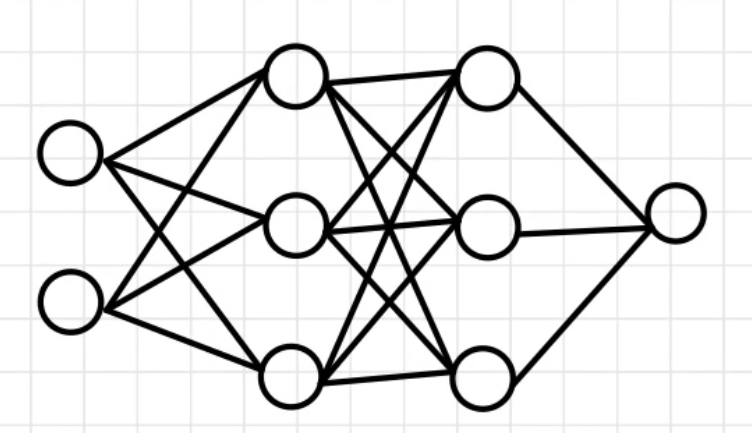
\includegraphics[width=8cm]{./capture/confirm_test/day1_01_1.png}
  \caption{入力層2ノード1層・中間層3ノード2層・出力層1ノード1層のネットワーク}
  \label{fig:2-3-1}
\end{figure}

\par
ニューラルネットワークは、自動売買・チャットボット・画像認識・音声認識・自然言語処理・囲碁将棋AIなど、多くの分野で利用されている。
\par
ニューラルネットワークの1つのノードに対して、入力$x_i$, 重み$w_i$, バイアス$b$, 総入力$u$, 出力$z$, 活性化関数$f$とすると、
\begin{align}
  u &= \sum_{i=1}^{n}w_ix_i + b \\
  z &= f(u)
\end{align}
で表される。この出力は次のノードの入力として用いられることになる。
\begin{itembox}[l]{確認テスト}
  Q: 図\ref{fig:day1_02_1}に動物分類の実例を入れろ。

  A: 図\ref{fig:day1_02_2}を参照

  Q: 図\ref{fig:day1_02_3}の数式を書け。

  A: 図\ref{fig:day1_02_4}を参照
\end{itembox}
\begin{figure}[ht]
    \centering
    \begin{subfigure}[b]{0.45\textwidth}
      \centering
      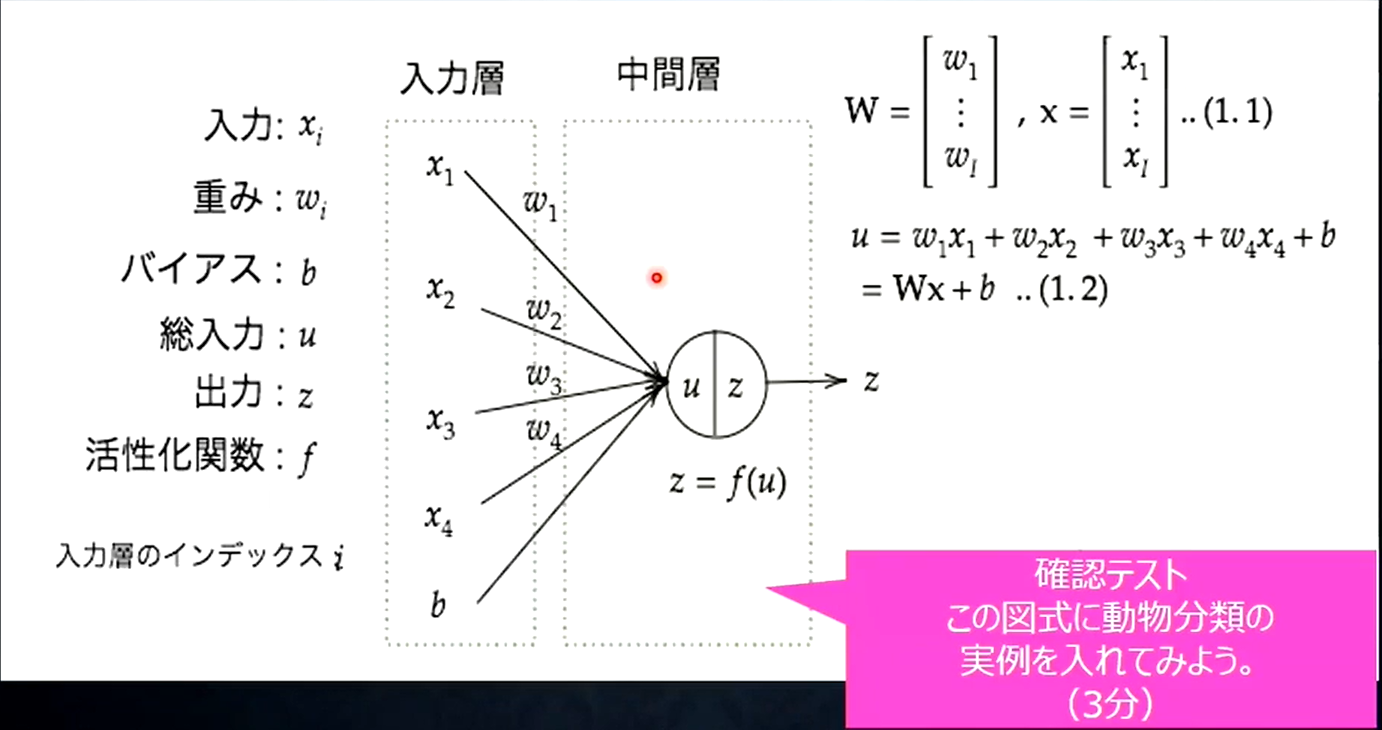
\includegraphics[width=\textwidth]{./capture/confirm_test/day1_02_1.png}
      \caption{}
      \label{fig:day1_02_1}
    \end{subfigure}
    \hfill
    \begin{subfigure}[b]{0.45\textwidth}
      \centering
      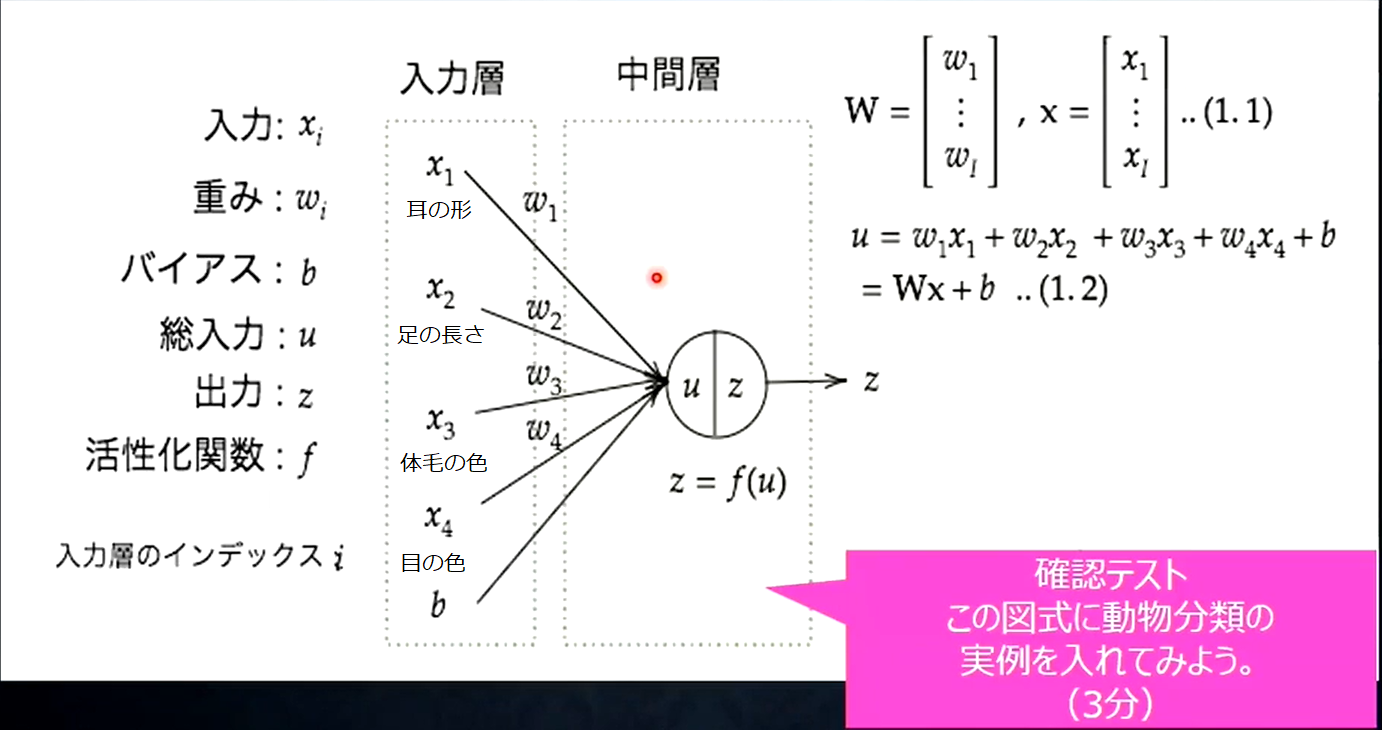
\includegraphics[width=\textwidth]{./capture/confirm_test/day1_02_2.png}
      \caption{}
      \label{fig:day1_02_2}
    \end{subfigure}
    \caption{}
\end{figure}

\begin{figure}[ht]
  \centering
  \begin{subfigure}[b]{0.45\textwidth}
    \centering
    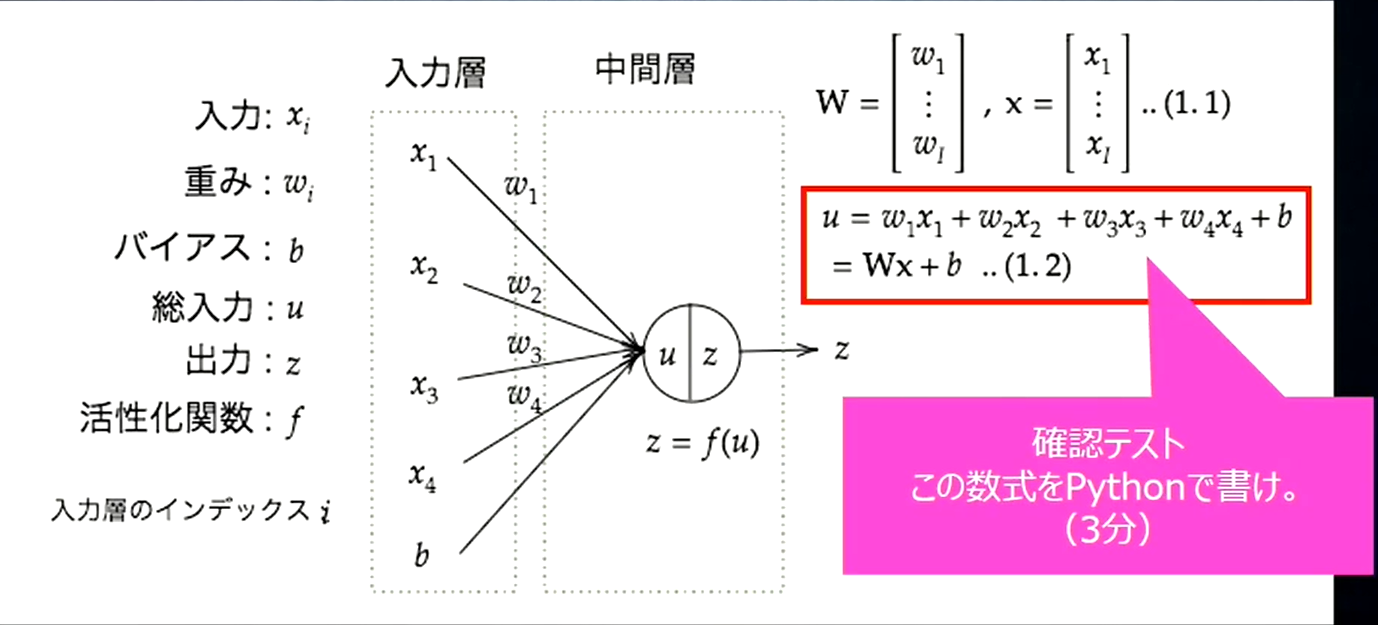
\includegraphics[width=\textwidth]{./capture/confirm_test/day1_02_3.png}
    \caption{}
    \label{fig:day1_02_3}
  \end{subfigure}
  \hfill
  \begin{subfigure}[b]{0.45\textwidth}
    \centering
    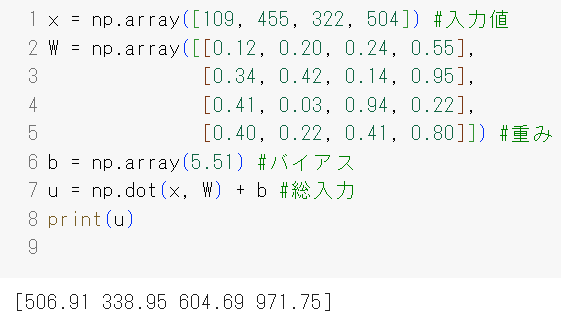
\includegraphics[width=\textwidth]{./capture/confirm_test/day1_02_4.png}
    \caption{}
    \label{fig:day1_02_4}
  \end{subfigure}
  \caption{}
\end{figure}

中間層と出力層で用いられる活性化関数に違いがある。
中間層では、ReLU関数、シグモイド関数、ステップ関数といった関数が用いられることが多い。
出力層では、ソフトマックス関数、シグモイド関数、恒等関数といった関数が用いられることが多い。
出力層において用いる活性化関数と誤差関数は、扱う問題に応じて選択する必要がある。
\begin{enumerate}
  \item 回帰問題の場合 → 恒等関数・二乗和誤差
  \item 2値分類問題の場合 → シグモイド関数・交差エントロピー誤差
  \item 多クラス分類問題の場合 → ソフトマックス関数・交差エントロピー誤差
\end{enumerate}

\subsection{活性化関数}
活性化関数とは、入力を出力に変換する関数である。活性化関数には、ステップ関数・シグモイド関数・ReLU関数・恒等関数・ソフトマックス関数などがある。
\subsubsection{ステップ関数}
閾値を超えたら発火する関数で、0か1を示す。
Pythonのサンプルコードを示す。
\begin{screen}
  \begin{verbatim}
    def step_function(x):
        if x > 0:
            return 1
        else:
            return 0
  \end{verbatim}
\end{screen}

\subsubsection{シグモイド関数}
勾配消失問題がある関数で、0から1の値を示す。
Pythonのサンプルコードを示す。
\begin{screen}
  \begin{verbatim}
    def sigmoid(x):
        return 1 / (1 + np.exp(-x))
  \end{verbatim}
\end{screen}


\subsubsection{ReLU関数}
勾配消失問題を回避し、スパース化によって過学習を防ぐ関数である。
Pythonのサンプルコードを示す。
\begin{screen}
  \begin{verbatim}
    def relu(x):
        return np.maximum(0, x)
  \end{verbatim}
\end{screen}


\subsubsection{恒等関数}
入力をそのまま出力する関数である。
Pythonのサンプルコードを示す。
\begin{screen}
  \begin{verbatim}
    def identity_function(x):
        return x
  \end{verbatim}
\end{screen}

\begin{itembox}[l]{確認テスト}
  Q: 図\ref{fig:day1_03_1}の赤枠に該当する箇所をソースコードから抜き出せ。

  A: 図\ref{fig:day1_03_2}を参照
\end{itembox}

\begin{figure}[ht]
  \centering
  \begin{subfigure}[b]{0.45\textwidth}
    \centering
    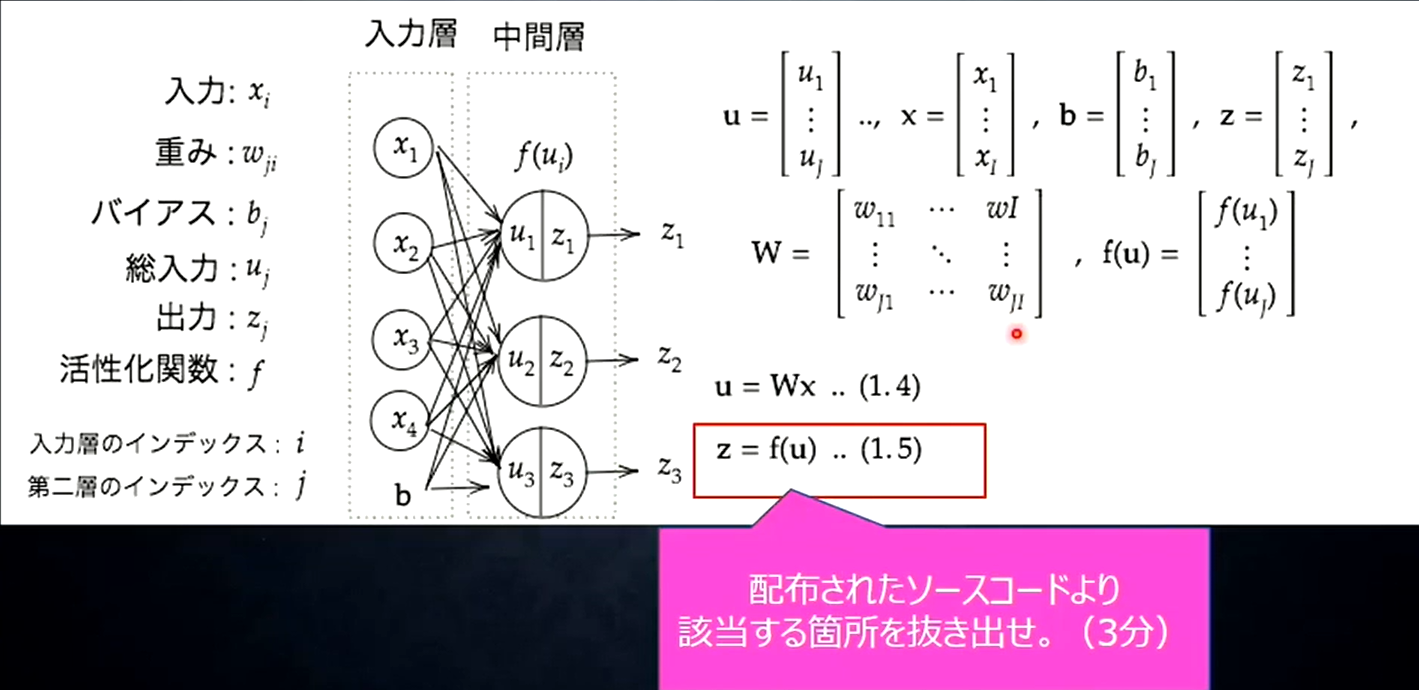
\includegraphics[width=\textwidth]{./capture/confirm_test/day1_03_1.png}
    \caption{}
    \label{fig:day1_03_1}
  \end{subfigure}
  \hfill
  \begin{subfigure}[b]{0.45\textwidth}
    \centering
    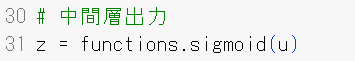
\includegraphics[width=\textwidth]{./capture/confirm_test/day1_03_2.png}
    \caption{}
    \label{fig:day1_03_2}
  \end{subfigure}
  \caption{}
\end{figure}

\subsubsection{ソフトマックス関数}
出力の総和が1になる関数である。
数式で表すと、以下の通りとなる。
\begin{align}
  f(i,u) = \frac{\exp(u_i)}{\sum_{k=1}^{K}\exp(u_k)}
\end{align}
Pythonのサンプルコードを示す。
\begin{screen}
  \begin{verbatim}
    def softmax(x):
        return np.exp(x) / np.sum(np.exp(x))
  \end{verbatim}
\end{screen}

\begin{itembox}[l]{確認テスト}
  Q: 図\ref{fig:day1_05_1}の丸1から丸3までの数式に該当するソースコードを示し、1行ずつ処理の説明をせよ。

  A: 図\ref{fig:day1_05_2}を参照。それぞれの説明は以下の通り。
  \begin{itemize}
    \item[①.] 2層目の総出力$u_2$を入力として、ソフトマックス関数を適用する。
    \item[②.] ソフトマックス関数の分子を計算する。
    \item[③.] ソフトマックス関数の分母を計算する。
  \end{itemize}
  
\end{itembox}

\begin{figure}[ht]
  \centering
  \begin{subfigure}[b]{0.45\textwidth}
    \centering
    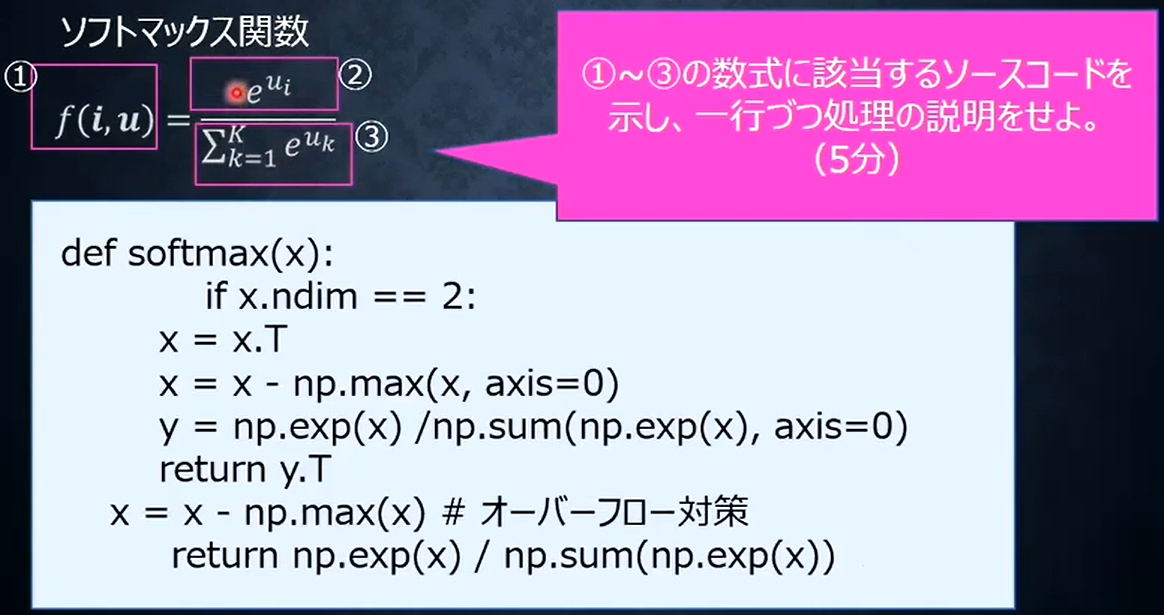
\includegraphics[width=\textwidth]{./capture/confirm_test/day1_05_1.png}
    \caption{}
    \label{fig:day1_05_1}
  \end{subfigure}
  \hfill
  \begin{subfigure}[b]{0.45\textwidth}
    \centering
    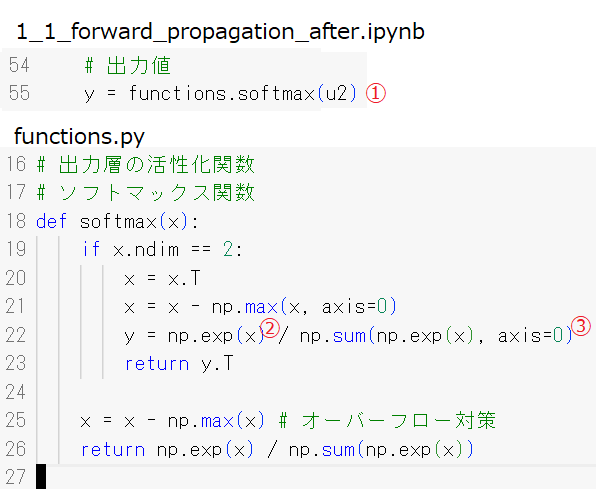
\includegraphics[width=\textwidth]{./capture/confirm_test/day1_05_2.png}
    \caption{}
    \label{fig:day1_05_2}
  \end{subfigure}
  \caption{}
\end{figure}

\subsection{誤差関数}
\subsubsection{二乗和誤差}
二乗和誤差とは、予測値と正解値の差の2乗和を2で割ったものである。
数式で表すと、以下の通りとなる。
\begin{align}
  E(\mathbf{w}) = \frac{1}{2}\sum_{i=1}^{w}(y_i - t_i)^2
\end{align}

\begin{itembox}[l]{確認テスト}
  Q: 二乗和誤差は、なぜ単なる引き算ではなく二乗するのか述べよ。
  
  A: 二乗和誤差は、予測値と正解値の差を取ることで、正解値との誤差を表す。二乗することで、正解値との誤差が大きい場合に誤差が大きくなり、正解値との誤差が小さい場合に誤差が小さくなるようにするためである。

  Q : 二乗和誤差の$\frac{1}{2}$はどういう意味を持つか述べよ。

  A: $\sum_{i=1}^{w} (y_i-t_i)^2$の微分値は以下の通りである。
  \begin{align}
    \frac{\partial E}{\partial y_i} &= \frac{\partial}{\partial y_i}\left( \sum_{i=1}^{n}(y_i - t_i)^2 \right) \\
    &= 2(y_i - t_i)
  \end{align}
  二乗和誤差の定義式で$\frac{1}{2}$を掛けるのは、前に出た2を消し、微分値を$(y_i - t_i)$として、計算を簡単にするためである。
\end{itembox}

\begin{itembox}{平均二乗和誤差と二乗和誤差}
機械学習でよく用いられる平均二乗誤差(Mean Squared Error: MSE)は、二乗和誤差の分母2をデータ数に変えて計算したものである。数式で表すと、以下の通りとなる。
\begin{align}
  E(\mathbf{w}) = \frac{1}{n}\sum_{i=1}^{w}(y_i - t_i)^2
\end{align}
平均二乗和誤差は、データ数によって誤差のスケールが変わるため、データ数が異なる場合でも誤差を比較することができる。
一方で、二乗和誤差は、データ数によって誤差のスケールが変わらないため、データ数が異なる場合は誤差を比較することができないが、計算が簡単という特徴がある。
\end{itembox}

\subsubsection{交差エントロピー誤差}
交差エントロピー誤差とは、2つの確率分布の違いを表す指標である。
数式で表すと、以下の通りとなる。
\begin{align}
  E(\mathbf{w}) = -\sum_{i=1}^{w} t_i log(y_i)
\end{align}
ただし、$t_i$は正解ラベル、$y_i$は予測値を表す。
この式を例を示しながら説明する。
写真に写っている動物が犬であるとする。
分類器は、犬・猫・ネズミを見分けることができるとし、いずれかのクラスの確率を出力する。
今、犬・猫・ネズミのそれぞれの確率を0.8, 0.1, 0.1であると予測した場合、交差エントロピー誤差は、
\begin{align}
  E &= -1.0*\log(0.8) - 0.0*\log(0.1) - 0.0*\log(0.1) \\
   &= 0.223
\end{align}
となる。次に、犬・猫・ネズミのそれぞれの確率を0.4, 0.3, 0.3 であると予測した場合、交差エントロピー誤差は、
\begin{align}
  E &= -1.0*\log(0.4) - 0.0*\log(0.3) - 0.0*\log(0.3) \\
   &= 0.52
\end{align}
となる。このように、交差エントロピー誤差は、予測が正解に近いほど小さくなり、予測が不正解に近いほど大きくなる。これは直観的にも誤差関数として交差エントロピー誤差が適していることが分かる。

\begin{itembox}[l]{確認テスト}
  Q: 図\ref{fig:day1_05_3}の丸1から丸2までの数式に該当するソースコードを示し、1行ずつ処理の説明をせよ。

  A: 図\ref{fig:day1_05_4}を参照。それぞれの説明は以下の通り。
  \begin{itemize}
    \item[①.] 正解値$d$, 予測値$y$を入力を与えて、交差エントロピー誤差を呼び出す。 
    \item[②.] $\log{y^d} = d\log{y}$として、numpyのlog関数を用いて計算する。1.0d-7を加えるのは、log(0)を防ぐためである。
  \end{itemize}
  
\end{itembox}

\begin{figure}[ht]
  \centering
  \begin{subfigure}[b]{0.45\textwidth}
    \centering
    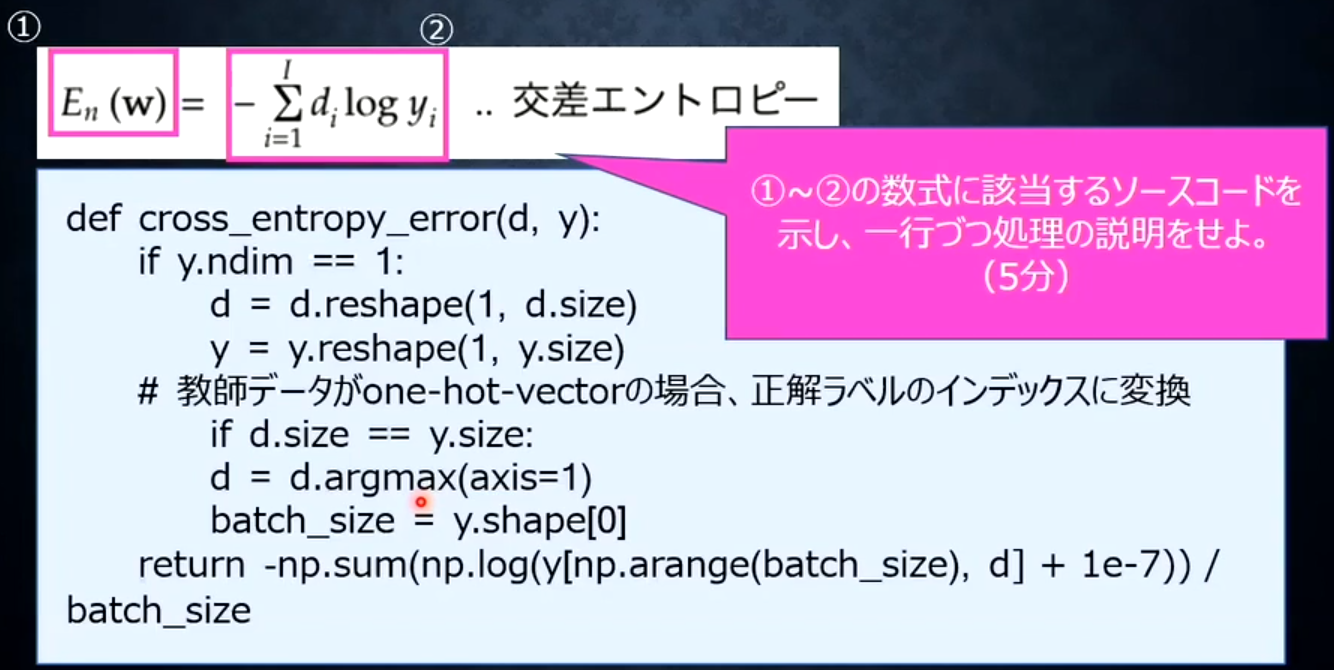
\includegraphics[width=\textwidth]{./capture/confirm_test/day1_05_3.png}
    \caption{}
    \label{fig:day1_05_3}
  \end{subfigure}
  \hfill
  \begin{subfigure}[b]{0.45\textwidth}
    \centering
    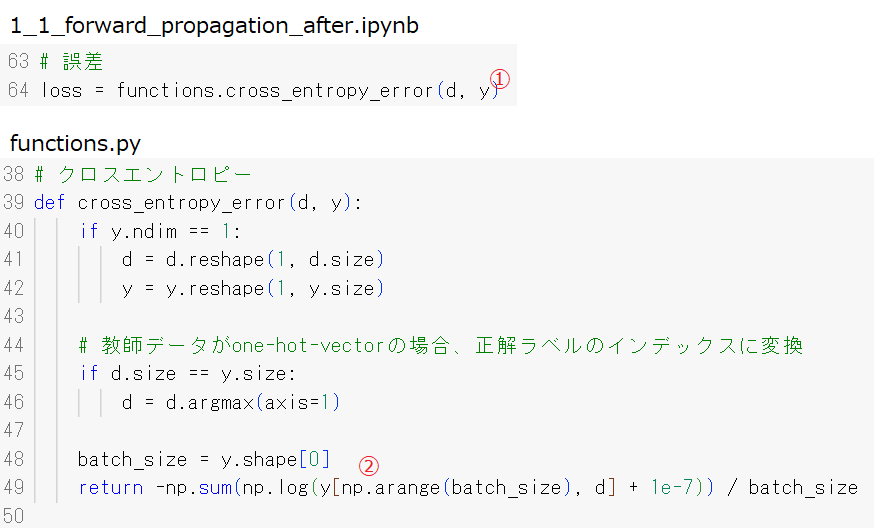
\includegraphics[width=\textwidth]{./capture/confirm_test/day1_05_4.png}
    \caption{}
    \label{fig:day1_05_4}
  \end{subfigure}
  \caption{}
\end{figure}

\subsubsection{カテゴリカル交差エントロピー誤差}
カテゴリカル交差エントロピー誤差とは、多クラス分類問題において用いられる誤差関数である。
数式で表すと、以下の通りとなる。
\begin{align}
  E= -\sum_{j=1}^{L-1} \sum_{i=1}^{M-1} t_{ji} \log(y_{ji})
\end{align}
ただし、$t_i$は正解ラベル、$y_i$は予測値、$L$はクラス数、$M$はクラス数を表す。
交差エントロピー誤差をクラス間で拡張し、すべてを足し合わせている。


\subsection{勾配降下法}
勾配降下法とは、導関数を用いて数値的に方程式の解を求めるための方法である。
深層学習では、学習を通して誤差関数を最小にするパラメータ$\mathbf{w}$を求めることが目的であり、勾配降下法はそのための手法の一つとして用いられる。
勾配降下法は、以下の手順で行われる。
\begin{enumerate}
  \item パラメータ$\mathbf{w}$を初期化する
  \item 誤差関数$E(\mathbf{w})$を最小化するために、$\mathbf{w}$を更新する
  \item 収束するまで2を繰り返す
\end{enumerate}
数式で表すと、以下の通りとなる。
\begin{align}
  \label{eq:gradient_descent}
  \mathbf{w}^{(t+1)} = \mathbf{w}^{(t)} - \epsilon E(\mathbf{w})
\end{align}
ここで、$\epsilon$は学習率を表す。
学習率は、パラメータの更新量を調整するためのハイパーパラメータであり、大きすぎると発散し、小さすぎると収束が遅くなるため、適切な値を設定する必要がある。
勾配降下法には様々な種類があり、Momentum・AdaGrad・Adadelta・Adamなどがある。
\begin{itembox}[l]{確認テスト}
  Q: 式\eqref{eq:gradient_descent}に該当するソースコードを示せ。

  A: 図\ref{fig:day1_06_1}を参照
\end{itembox}

\begin{figure}[ht]
  \centering
  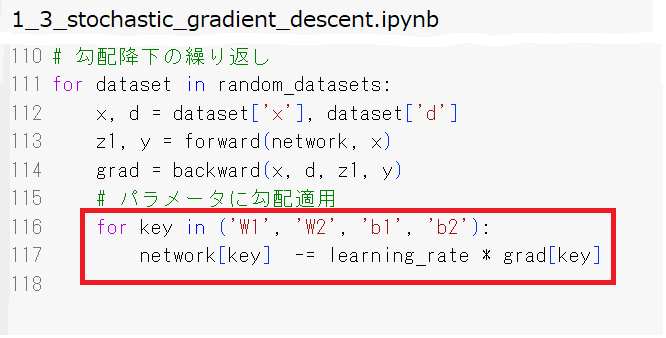
\includegraphics[width=10cm]{./capture/confirm_test/day1_06_1.png}
  \caption{}
  \label{fig:day1_06_1}
\end{figure}

\subsection{確率的勾配降下法(SGD)}
確率的勾配降下法とは、勾配降下法の一種であり、毎回違う学習データをランダムに選んで行う方法である。
計算コストを下げたり、局所解に陥ることを防ぐために用いられる。
勾配降下法を用いた深層学習モデルの学習データの選び方は、
\begin{enumerate}
  \item バッチ学習
  \item ミニバッチ学習
  \item オンライン学習
\end{enumerate}
の3つが挙げられる。
\par
バッチ学習は、エポック毎に全てのデータを使って傾きを逐次求め、最適解を見つける方法である。学習結果が安定しやすいという特徴を持つ。新たな訓練データが追加された場合に、再度全データを用いて計算を行う必要があるため、計算コストが高い。
\par
ミニバッチ学習は、すべてのデータの中から一部を取り出して学習する方法で、局所最適解を回避しやすいという特徴を持つ。バッチ学習とオンライン学習の中間の特徴を持つ。すべてのデータで学習し終えた時に1エポックが終了し、重みが更新される。
\par
オンライン学習は、すべてのデータの中から1つを取り出して学習する方法で、ミニバッチ学習よりも局所最適解を回避しやすいという特徴を持つ。計算コストが低いが、学習結果が不安定であるという特徴を持つ。
\par
深層学習のモデリングにおいては、ミニバッチ学習が最も一般的に用いられる。
その理由として、確率的勾配法のメリットを損なわずに、計算資源を有効利用することができるからである。
例えば、1000万件の学習データがあった場合、それをバッチ学習で学習しようとすると、1000万件のデータを一度に計算する必要がある。現代のコンピュータでは、1000万件のデータの計算には莫大な時間を要してしまう。そのため1000件ずつのミニバッチを作成し、それを10000回繰り返す際に、他の資源でも同時平行で計算することで時間を短縮させる。これには、CPUのスレッド並列化やGPUのSIMD並列化という技術が用いられる。

\begin{itembox}[l]{確認テスト}
  Q: $\mathbf{w^{(t+1)}} = \mathbf{w^{(t)}} - \epsilon \nabla E_t$ の数式の意味を図に書いて説明せよ。

  A: 図\ref{fig:day1_08_1}を参照
\end{itembox}

\begin{figure}[ht]
  \centering
  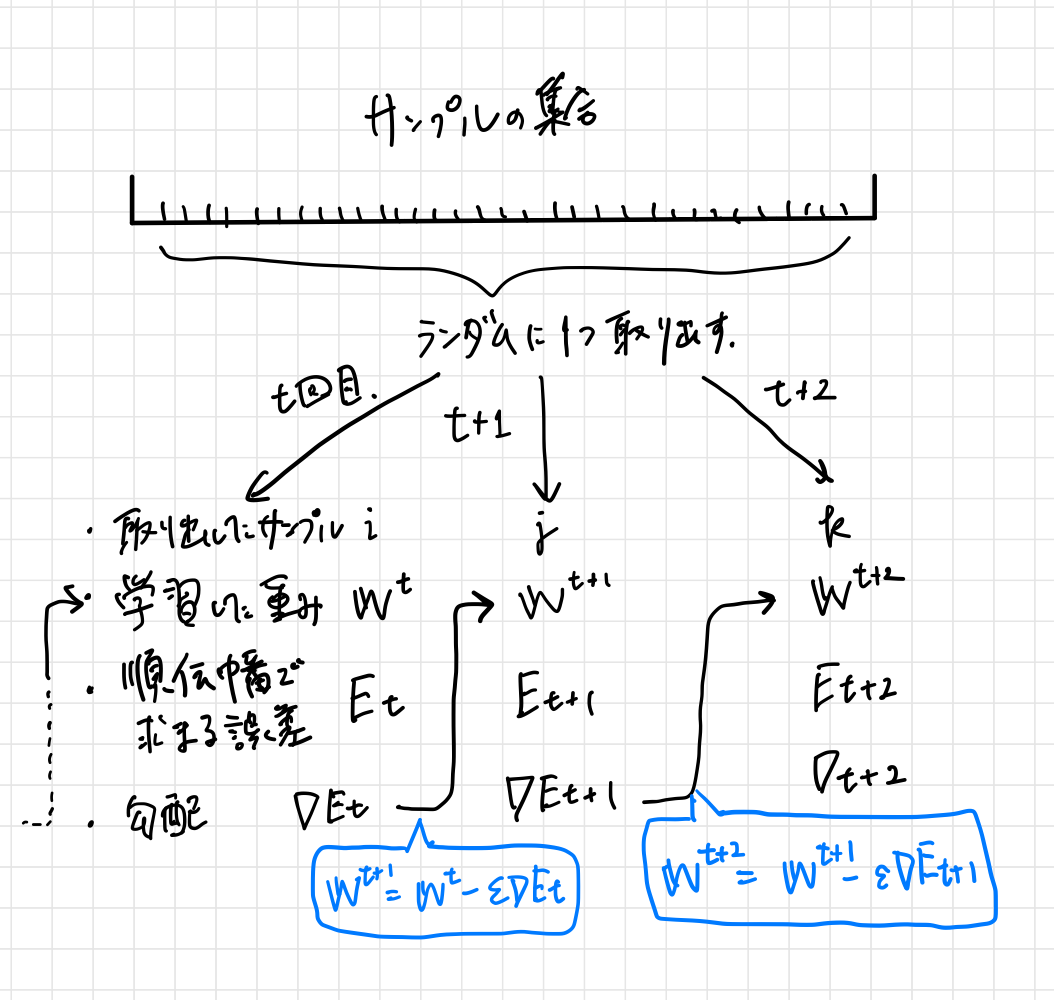
\includegraphics[width=10cm]{./capture/confirm_test/day1_08_1.png}
  \caption{}
  \label{fig:day1_08_1}
\end{figure}

\subsection{誤差逆伝播法}
勾配降下法を用いて、重みとバイアスを更新する際に用いられる方法が誤差逆伝播法である。
誤差逆伝播法は、出力層から入力層に向かって、誤差を逆伝播させることで、各層の重みとバイアスを更新する方法である。
誤差逆伝播法は、以下の手順で行われる。
\begin{enumerate}
  \item 順伝播
  \item 誤差逆伝播
  \item 重みとバイアスの更新
\end{enumerate}
数式で表すと、以下の通りとなる。
\begin{align}
  w &\leftarrow w - \epsilon \frac{\partial E}{\partial w} \\
  b &\leftarrow b - \epsilon \frac{\partial E}{\partial b}
\end{align}
ただし、$w$は重み、$b$はバイアス、$\epsilon$は学習率、$E$は誤差関数を表す。
勾配を求めることができれば、上式を用いて重みとバイアスを更新することができる。

以下では、ノード$i$における前ノード$j$との間の重み$w_{ij}$の勾配を求める。
まず、$\frac{\partial E}{\partial w_{ij}}$を求める。
\begin{align}
  \frac{\partial E}{\partial w_{ij}} = \frac{\partial E}{\partial u_i}\frac{\partial u_i}{\partial w_{ij}}
\end{align}
$u_i$は、ノード$i$の総入力を表し、
\begin{align}
  u_i = \sum_{j=1}^{m}w_{ij}y_j + b_i
\end{align}
であるから、$\frac{\partial u_i}{\partial w_{ij}}$は、
\begin{align}
  \frac{\partial u_i}{\partial w_{ij}} &= \frac{\partial}{\partial w_{ij}}\left( \sum_{j=1}^{m}w_{ij}y_j + b_i \right)\\
   &= y_j
\end{align}
となる。また、$\frac{\partial E}{\partial u_i}$は、
\begin{align}
  \frac{\partial E}{\partial u_i} = \frac{\partial E}{\partial y_i}\frac{\partial y_i}{\partial u_i}
\end{align}
で表される。ここで、$E$が二乗和誤差の場合、
\begin{align}
  \frac{\partial E}{\partial y_i} &= \frac{\partial}{\partial y_i}\left( \frac{1}{2} \left( \sum_{i=1}^{n}(y_i - t_i)^2 \right) \right) \\
  &= y_i - t_i
\end{align}
となる。また、$y_i$が恒等関数の場合、
\begin{align}
  \frac{\partial y_i}{\partial u_i} &= \frac{\partial}{\partial u_i}u_i \\
  &= 1
\end{align}
となる。以上より、$\frac{\partial E}{\partial u_i}$は、
\begin{align}
  \frac{\partial E}{\partial u_i} = (y_i - t_i) \times 1 = y_i - t_i
\end{align}
となる。よって、$\frac{\partial E}{\partial w_{ij}}$は、
\begin{align}
  \frac{\partial E}{\partial w_{ij}} = (y_i - t_i)y_j
\end{align}
となる。同様に、バイアス$b_i$についても、
\begin{align}
  \frac{\partial E}{\partial b_i} = \frac{\partial E}{\partial u_i}\frac{\partial u_i}{\partial b_i} = y_i - t_i
\end{align}
となる。以上より、重みとバイアスの更新式は、
\begin{align}
  w_{ij} &\leftarrow w_{ij} - \epsilon(y_i - t_i)y_j \\
  b_i &\leftarrow b_i - \epsilon(y_i - t_i)
\end{align}
となる。これを、ノード$i$におけるすべての前ノード$j$について計算するために、行列表現で表すと、
\begin{align}
  \mathbf{w} &\leftarrow \mathbf{w} - \epsilon \mathbf{y}^T(y_i - t_i) \\
  \mathbf{b} &\leftarrow \mathbf{b} - \epsilon(y_i - t_i)
\end{align}
となる。ここで、$\mathbf{y}$を転置しているのは、$\mathbf{w}$と形状を合わせるためである。

図\ref{fig:backprop}に、誤差逆伝播の概要を示す。
\begin{figure}[htbp]
  \centering
  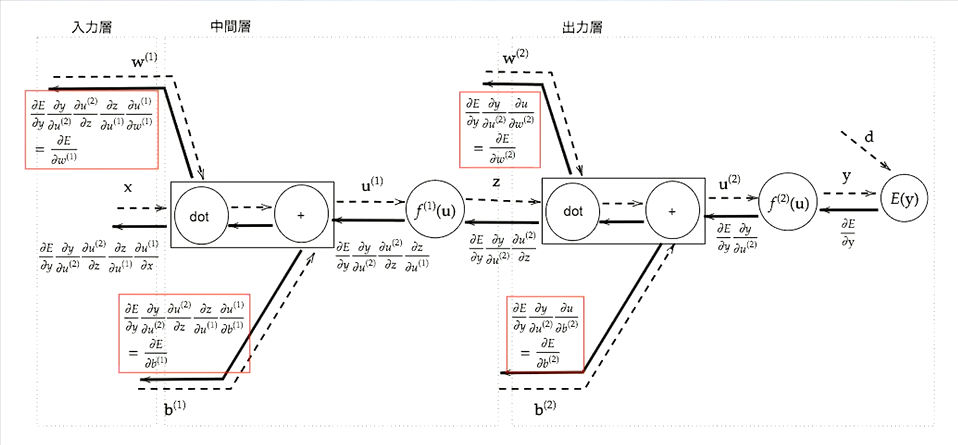
\includegraphics[width=13cm]{./capture/backprop.png}
  \caption{誤差逆伝播法における勾配}
  \label{fig:backprop}
\end{figure}

\newpage

\begin{itembox}[l]{確認テスト}
  Q: 誤差逆伝搬法では不要な再帰的処理を避けることができる。すでに行った計算結果を保持しているソースコードを抽出せよ。

  A: 図\ref{fig:day1_10_1}を参照

  Q: $\frac{\partial E}{\partial y} \frac{\partial y}{\partial u}$と、$\frac{\partial E}{\partial y} \frac{\partial y}{\partial u} \frac{\partial u}{\partial w_{ji}^{(2)}}$に該当するソースコードを探せ。

  A: 図\ref{fig:day1_10_2}を参照
\end{itembox}

\begin{figure}[ht]
  \centering
  \begin{subfigure}[b]{0.45\textwidth}
    \centering
    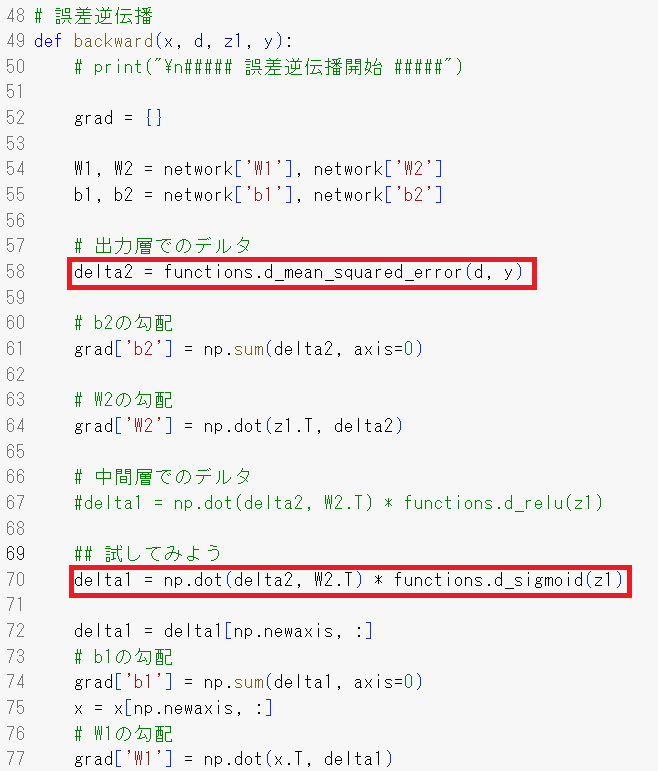
\includegraphics[width=\textwidth]{./capture/confirm_test/day1_10_1.png}
    \caption{}
    \label{fig:day1_10_1}
  \end{subfigure}
  \hfill
  \begin{subfigure}[b]{0.45\textwidth}
    \centering
    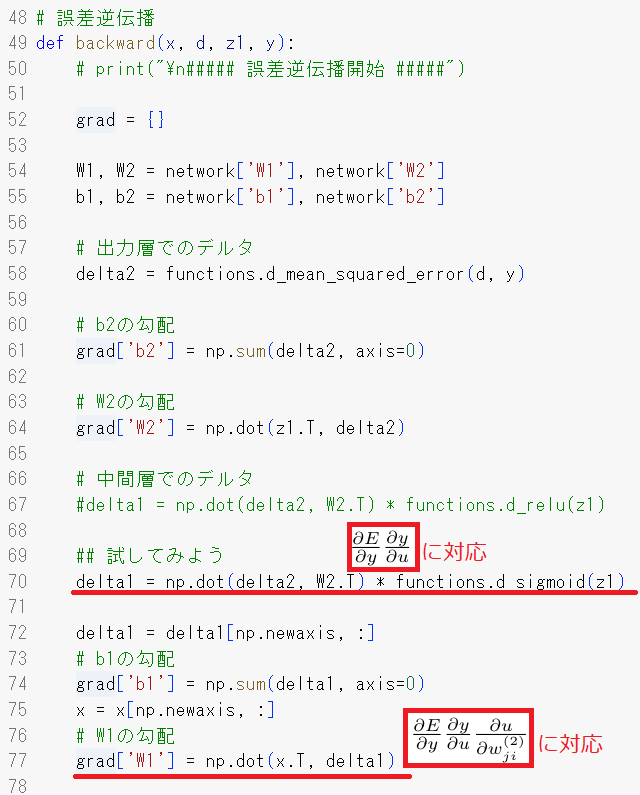
\includegraphics[width=\textwidth]{./capture/confirm_test/day1_10_2.png}
    \caption{}
    \label{fig:day1_10_2}
  \end{subfigure}
  \caption{}
\end{figure}

\newpage

\begin{itembox}[l]{計算グラフ}
  計算グラフとは計算の過程をグラフで視覚化したものである。これを用いることで、複雑な偏微分の連なりを分解し、出力へ影響を与えるノードを絞りこむことができるようになる。
  計算グラフは複数の「ノード」と「エッジ」から構成される。
  例えば、a,b,c,d,e,fをノードとし、
  \begin{align}
    e = ab\\
    f = cd\\
    g = e + f
  \end{align}
  を計算グラフで表すと、図\ref{fig:calc_graph}の青字ようになる。これは順伝播を表す。
  \par
  ここで、最終的な出力である$g$が、それぞれのノードの影響をどの程度受けるか知りたいとする。
  偏微分について以下が成立することは明白である。
  \begin{align}
    f(a,b) &= ab\\
    \frac{\partial f}{\partial a} &= b\\
    \frac{\partial f}{\partial b} &= a\\
    g(e,f) &= e + f\\
    \frac{\partial g}{\partial e} &= 1\\
    \frac{\partial g}{\partial f} &= 1
  \end{align}
  $e, f$は、値の大きさに依らずそれぞれ1の影響を$g$に与える。つまり、$e$の値が1変わったら$g$が1変わるという意味である。
  $a, b, c, d$は、$e, f$に対してそれぞれ2, 3, 5, 4の影響を与える。これらは同様に、$a, b, c, d$の値が1変わったら、$e, f$がそれぞれ2, 3, 5, 4変わるという意味である。さらに$e, f$は$g$に等倍の影響であるため、$a, b, c, d$が1変わったら、$g$が$2+3+5+4=14$変わることがわかる。これらの処理の流れは、図\ref{fig:calc_graph}の黄色で示されており、逆伝播を表す。
  \par
  ここでは、計算グラフを用いることで、$g$に与える影響が最も大きいノードは$c$であることが分かった。

\end{itembox}

\begin{figure}[htbp]
  \centering
  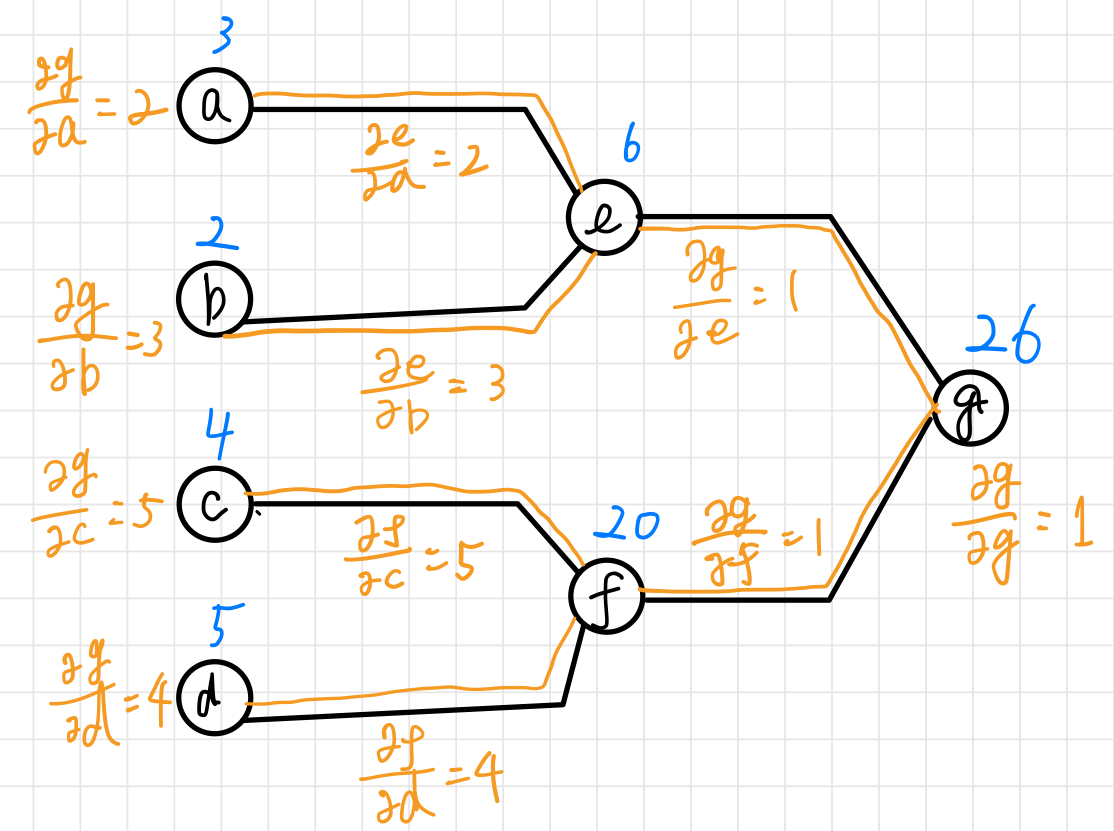
\includegraphics[width=8cm]{./capture/calc_graph.png}
  \caption{計算グラフ}
  \label{fig:calc_graph}
\end{figure}

\begin{figure}[htbp]
  \centering
  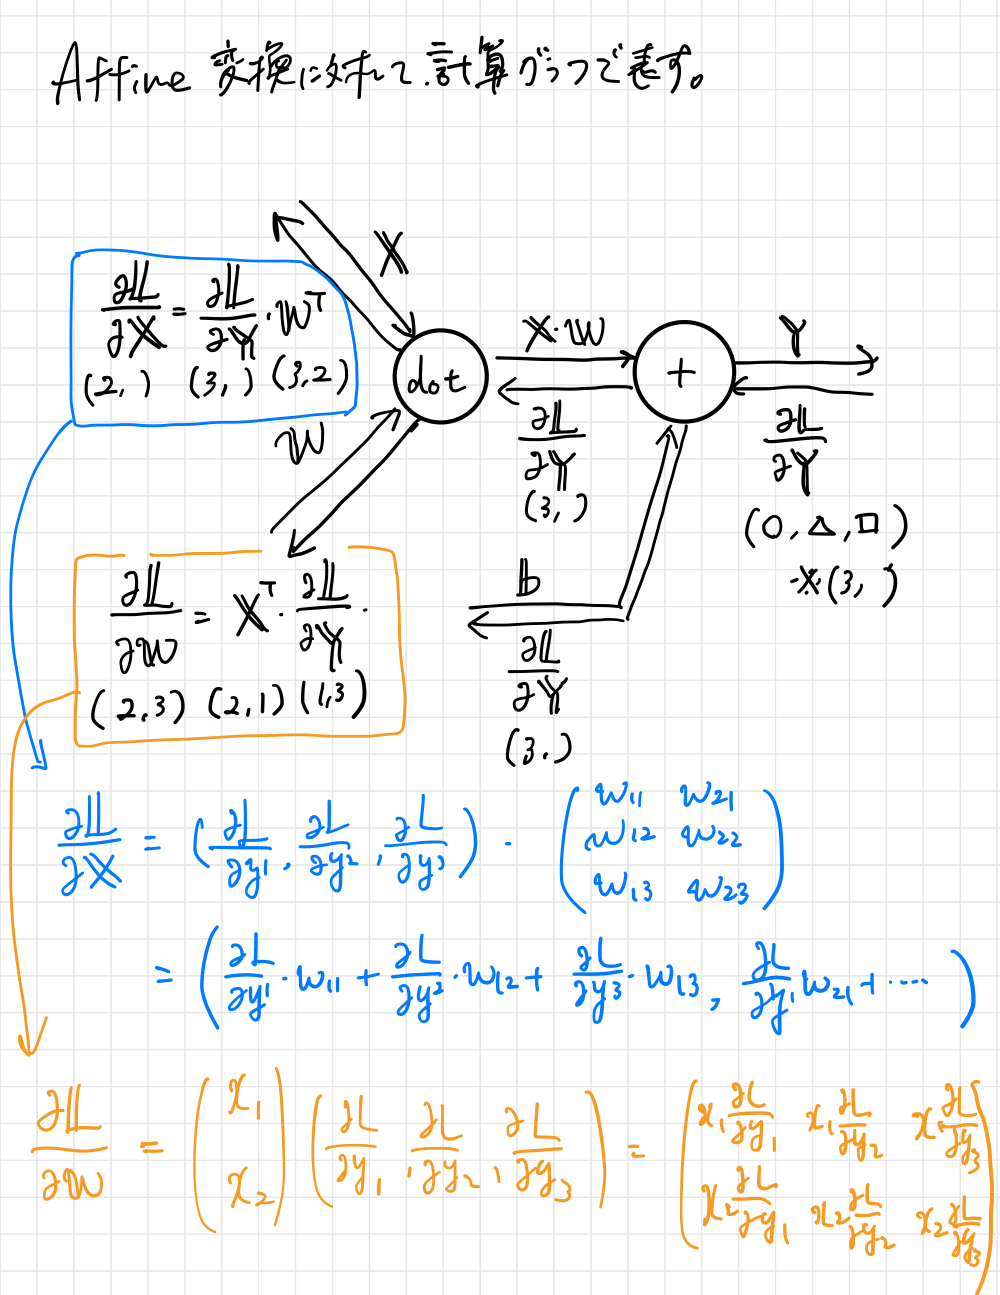
\includegraphics[width=8cm]{./capture/affine_calc_graph.png}
  \caption{Affine変換を計算グラフで表す}
  \label{fig:affine_calc_graph}
\end{figure}
  
\newpage

\section{Day2 : ニューラルネットワーク}
\subsection{勾配消失問題}
勾配消失問題とは、多層ニューラルネットワークにおいて、勾配が逆伝播する際に、勾配が小さくなり、学習が進まなくなる問題である。
勾配消失問題は、シグモイド関数やハイパボリックタンジェント関数を活性化関数として用いた場合に発生しやすい。
シグモイド関数の微分は、
\begin{align}
  \frac{d}{dx}\sigma(x) = \sigma(x)(1 - \sigma(x))
\end{align}
であり、これをグラフにすると、最大値が0.25であることがわかる。
図\ref{fig:backprop}において、活性化関数$f(u)$をシグモイド関数として考えた時、$u$の更新式である、
\begin{align}
  u^{(3)} &\leftarrow u - \epsilon \frac{\partial E}{\partial y}\frac{\partial y}{\partial u}\\
  u^{(2)} &\leftarrow u - \epsilon \frac{\partial E}{\partial y}\frac{\partial y}{\partial u^{(3)}} \frac{\partial u^{(3)}}{\partial z^{(2)}} \frac{\partial z^{(2)}}{\partial u^{(2)}}\\
  u^{(1)} &\leftarrow u - \epsilon \frac{\partial E}{\partial y} \frac{\partial y}{\partial u^{(3)}} \frac{\partial u^{(3)}}{\partial z^{(2)}} \frac{\partial z^{(2)}}{\partial u^{(2)}} \frac{\partial u^{(2)}}{\partial z^{(1)}} \frac{\partial z^{(1)}}{\partial u^{(1)}}
\end{align}
における、$\frac{\partial y}{\partial u}, \frac{\partial z^{(2)}}{\partial u^{(2)}}, \frac{\partial z^{(1)}}{\partial u^{(1)}}$が最大値0.25の少数となる。模式図では中間層が1層のみであるが、実際にはさらに多くの層を持つため、これらの値が掛け合わされることで、勾配が指数関数的に小さくなり、勾配消失問題が発生する。
\par
勾配消失問題に対しては以下の3つの解決方法が考えられる。
\begin{enumerate}
  \item 活性化関数の選択
  \item 重みの初期値の設定
  \item バッチ正規化
\end{enumerate}

\subsubsection{活性化関数の選択}
活性化関数の選択については、ReLU関数やLeaky ReLU関数を用いることで、勾配消失問題を回避することができる。
Leaky ReLU関数は以下の数式で定義される。
\begin{align}
  f(x) = \begin{cases}
    x & (x > 0)\\
    ax & (x \leq 0)
  \end{cases}
\end{align}
ここで、$a$は0より大きい小さな値である。
Leaky ReLU関数は、$x \leq 0$の時に、勾配が0にならず、$x$に比例して勾配が変化するため、勾配消失問題を回避することができる。
ReLU関数は、微分値が1になるため先ほどのシグモイド関数における問題が解消される。

\subsubsection{重みの初期値設定}
重みの初期値の設定については、活性化関数がsigmoidやtanhの場合Xavierの初期値、活性化関数がReLUの場合Heの初期値を用いることで、勾配消失問題を回避することができる。
\par
Xavierの初期値は、前の層のノード数を$n$とした時、標準偏差が$\frac{1}{\sqrt{n}}$の分布を用いて、対象の層と前の層の間の重みを初期化する方法である。
\par
Heの初期値は、前の層のノード数を$n$とした時、標準偏差が$\frac{2}{\sqrt{n}}$の分布を用いて、対象の層と前の層の間の重みを初期化する方法である。
\subsubsection{バッチ正規化}
バッチ正規化は、最初の入力データの正規化だけでなく、各層の出力に対しても正規化することで、勾配消失問題を回避して汎化性能を上げる方法である。
バッチ正規化は、学習時と推論時で挙動が異なるため、学習時には、ミニバッチごとに正規化を行い、推論時には、全データを用いて正規化を行う必要がある。
バッチ正規化を行う際は、まずミニバッチの平均・分散を求める。
\begin{align}
  \mu_i &= \frac{1}{m}\sum_{i=1}^{m}x_i \text{  (平均)} \\
  \sigma_i^2 &= \frac{1}{m}\sum_{i=1}^{m}(x_i - \mu_i)^2 \text{  (分散)}
\end{align}
次に、正規化を行う。この時、$\epsilon$を加えることで、分母が0になるのを防ぐ。
\begin{align}
  \hat{x}_i &=\frac{\text{(各値の平均からの差)}}{\text{(標準偏差)}}\\
  &=  \frac{x_i - \mu_i}{\sqrt{\sigma_i^2 + \epsilon}} 
\end{align}
最後に、スケーリングとシフトを行う。
\begin{align} 
  y_i = \gamma \hat{x}_i + \beta
\end{align}
ここで、$\gamma$はスケーリング係数、$\beta$はシフト係数、$\epsilon$は微小値である。


\begin{itembox}[l]{確認テスト}
  Q: 重みの初期値を0に設定すると、どのような問題が発生するか。簡潔に説明せよ。

  A: 順伝播での出力がすべて同じ値となり、逆伝搬での勾配もすべて同じ値となるため、重みの更新がうまく行われず、学習が進まなくなる。

  Q: 一般的に考えられるバッチ正規化の効果を2点挙げよ。

  A: 学習データとテストデータの分布が異なる場合に、評価値を安定させる効果がある (汎化性能が上昇する)。また、勾配消失を解消して学習を早く進めることができる。
\end{itembox}



\subsection{学習率最適化手法}
学習率最適化手法とは、学習率を適切に設定するための手法である。学習率とは、重みの更新量を調整するためのハイパーパラメータであり、大きすぎると発散し、小さすぎると収束が遅くなるため、適切な値を設定する必要がある。
学習率最適化手法には、以下のような手法がある。
\begin{enumerate}
  \item モメンタム
  \item AdaGrad
  \item RMSProp
  \item Adam
\end{enumerate}

\subsubsection{モメンタム}
モメンタムは、勾配方向に加えて、前回の重みの更新量を考慮して、重みを更新する手法である。
モメンタムは、以下の式で表される。
\begin{align}
  v^{(t+1)} &= \epsilon \frac{\partial E}{\partial w} - \mu v^{(t)} \\
  w^{(t+1)} &= w^{(t)} - v^{(t+1)}
\end{align}
前回の重みの更新量に$\mu = 0.5 \sim 0.9$の値を掛け合わせたもの$v$を更新量として用いることで、勾配降下法における振動を抑える。よって、大域的最適解に向かって、谷の方向に沿って谷底を効率よく探索して収束していく特徴がある。

\subsubsection{AdaGrad(Adaptive Gradient Algorithm)}
AdaGradは、学習率を重みの要素ごとに変化させる手法である。
これまでの勾配の二乗和を経験としてすべて保持し、その経験に基づいて学習率を調整する。
AdaGradは、以下の式で表される。
\begin{align}
  h^{(t+1)} &= h^{(t)} + \left( \frac{\partial E}{\partial w} \right)^2 \\
  w^{(t+1)} &= w^{(t)} - \frac{\epsilon}{\sqrt{h^{(t+1)}}} \frac{\partial E}{\partial w}
\end{align}
AdaGradは、学習率が小さくなりすぎるという問題がある。
確かに、誤差関数の勾配が大きい場合、2つ目の式で、$\frac{1}{\sqrt{h^{(t+1)}}}$によって更新量が小さくなることが分かる。


\subsubsection{RMSProp}
RMSPropは、AdaGradの学習率が小さくなりすぎる問題を解決するために、指数移動平均を用いて、過去の勾配の影響を減衰させる手法である。
つまり、過去の経験を忘れることで、学習率が小さくなりすぎる問題を解決するということである。
RMSPropは、以下の式で表される。
\begin{align}
  h^{(t+1)} &= \alpha h^{(t)} + (1 - \alpha) \left( \frac{\partial E}{\partial w} \right)^2 \\
  w^{(t+1)} &= w^{(t)} - \frac{\epsilon}{\sqrt{h^{(t+1)}}} \frac{\partial E}{\partial w}
\end{align}
ここで、$\alpha$は減衰率を表すハイパーパラメータである。


\subsubsection{Adam}
Adamは、モメンタムの過去の勾配の指数関数的減衰平均と、RMSPropの二乗和の移動平均を組み合わせた手法である。
Adamは、以下の式で表される。
\begin{align}
  m^{(t+1)} &= \beta_1 m^{(t)} + (1 - \beta_1) \frac{\partial E}{\partial w} \\
  h^{(t+1)} &= \beta_2 h^{(t)} + (1 - \beta_2) \left( \frac{\partial E}{\partial w} \right)^2 \\
  \hat{m} &= \frac{m^{(t+1)}}{1 - \beta_1^{t+1}} \\
  \hat{h} &= \frac{h^{(t+1)}}{1 - \beta_2^{t+1}} \\
  w^{(t+1)} &= w^{(t)} - \frac{\epsilon}{\sqrt{\hat{h}} + \epsilon} \hat{m}
\end{align}
ここで、$\beta_1, \beta_2$はそれぞれモメンタムとRMSPropの減衰率を表すハイパーパラメータである。


\subsection{過学習}
過学習とは、学習データに対しては良い性能を示すが、テストデータに対しては性能が低くなる現象である。
深層学習モデルにおいて過学習が発生する原因は、以下の3つが挙げられる。
\begin{itemize}
  \item パラメータ数が多い
  \item データが少ない
  \item ノード数が多い
  \item → ネットワークの自由度が高いということ
\end{itemize}
過学習では、重みの行列の中で、極端に大きな値を持つものが現れてしまうことによって発生する。
過学習を防ぐためには、以下のような手法がある。
\begin{enumerate}
  \item 正則化
  \item ドロップアウト
  \item 早期終了
  \item データ拡張
\end{enumerate}

\subsubsection{正則化}
正則化は、過学習を防ぐために、誤差関数に正則化項を追加する手法である。
一般化されたL(N)正則化項は、以下の式で表される。
\begin{align}
  E(\mathbf{w}) + \frac{1}{p} \lambda ||\mathbf{w}||_p \\
  ||\mathbf{w}||_p = \left( \sum_{i=1}^{n}|w_i|^p \right)^{\frac{1}{p}}
\end{align}
ここで、$\lambda$は正則化項の重みを表すハイパーパラメータである。 
L1正則化は、$p=1$の場合であり、L2正則化は、$p=2$の場合である。
例えば、xとyの2次元のデータがある場合、L1正則化は、
\begin{align}
  |x| + |y|
\end{align}
となり、L2正則化は、
\begin{align}
  \sqrt{x^2 + y^2}
\end{align}
となる。
\begin{figure}
  \centering
  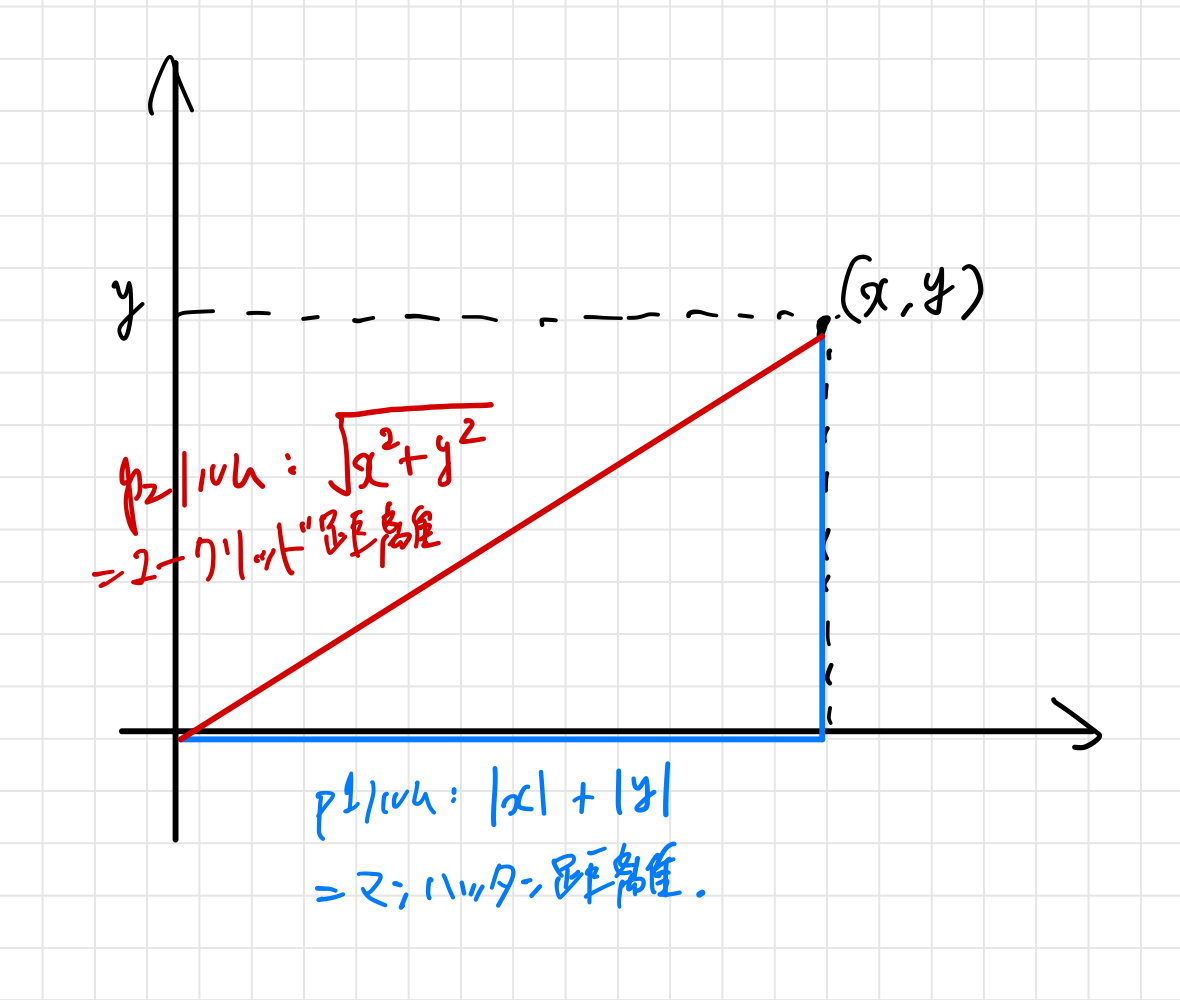
\includegraphics[width=10cm]{./capture/L1L2.png}
  \caption{L1, L2ノルムのイメージ}
\end{figure}
L1正則化を用いた回帰分析のことをLasso回帰と呼ぶ。Lasso回帰は、L1正則化を用いることで、スパースな解を得られやすいため、必要な特徴量のみを選択することができる (図\ref{fig:Lasso}) 。
L2正則化を用いた回帰分析のことをRidge回帰と呼ぶ。Ridge回帰は、L2正則化を用いることで、特徴量の重みを0に近づけることができるため、特徴量の重みを抑制することができる (図\ref{fig:Ridge}) 。

\begin{figure}[ht]
  \centering
  \begin{subfigure}[b]{0.45\textwidth}
    \centering
    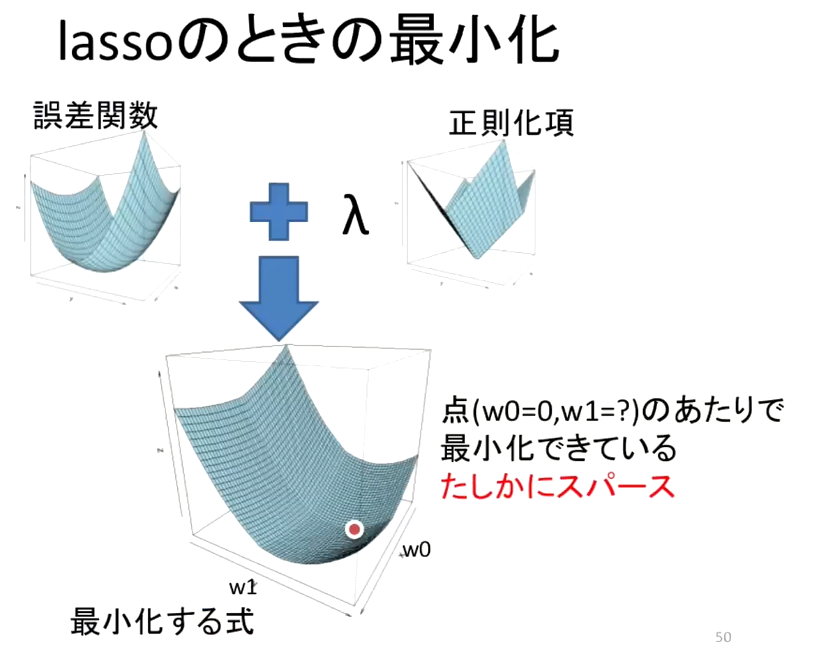
\includegraphics[width=\textwidth]{./capture/Lasso.png}
    \caption{Lasso回帰における正則化のイメージ (参照: 授業資料(Day2 18 過学習 正則化手法4))}
    \label{fig:Lasso}
  \end{subfigure}
  \hfill
  \begin{subfigure}[b]{0.45\textwidth}
    \centering
    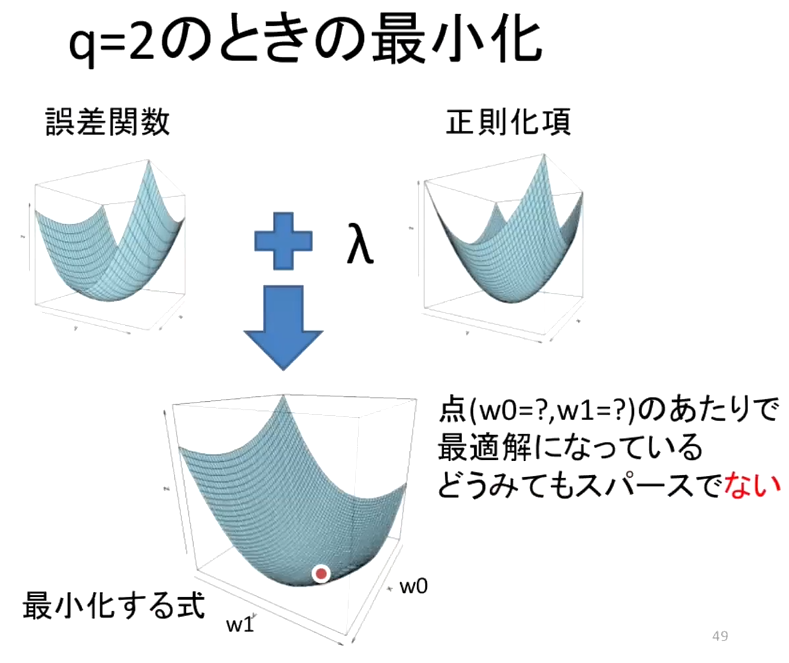
\includegraphics[width=\textwidth]{./capture/Ridge.png}
    \caption{Ridge回帰における正則化のイメージ (参照: 授業資料 Day2 18 過学習 正則化手法4))}
    \label{fig:Ridge}
  \end{subfigure}
  \caption{}
\end{figure}


\begin{itembox}[l]{確認テスト}
  Q: 図\ref{fig:day2_18_1}について、L1正則化を表しているグラフはどちらか答えよ。

  A: 順伝播での出力がすべて同じ値となり、逆伝搬での勾配もすべて同じ値となるため、重みの更新がうまく行われず、学習が進まなくなる。
\end{itembox}

\begin{figure}
  \centering
  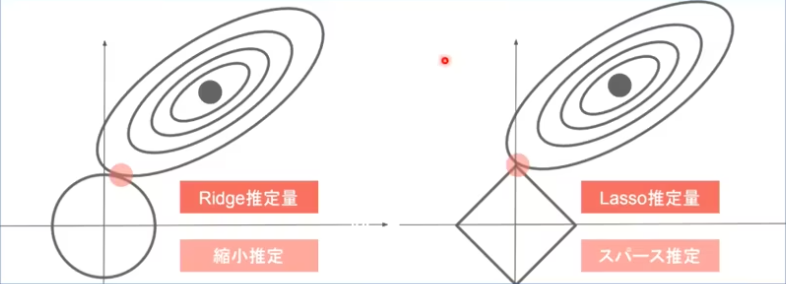
\includegraphics[width=10cm]{./capture/confirm_test/day2_18_1.png}
  \caption{}
  \label{fig:day2_18_1}
\end{figure}

\subsubsection{ドロップアウト}
ドロップアウトは、ニューラルネットワークの学習時に、ランダムにノードを削除することで、過学習を防ぐ手法である。
ドロップアウトは、以下の式で表される。
\begin{align}
  y_i = r_i \times x_i
\end{align}
ここで、$r_i$は、ノード$i$を削除する確率を表すハイパーパラメータである。
ドロップアウトは、学習時にのみ適用し、テスト時には適用しない。
ドロップアウトは、モデルの自由度を下げることで、過学習を防ぐ効果がある。


\newpage
\section{Day2 : 畳み込みニューラルネットワーク(CNN)}
\subsection{概要}
CNNは、画像認識や音声認識などの分野で高い性能を発揮するニューラルネットワークである。
ある画像に対しては、隣り合うピクセルの情報が似通う可能性が高い。また、ある動画に対しては、連続するフレームの画像情報が似通う可能性が高い。
そのような次元間で連続した情報を扱う際に、CNNは高い効果を発揮する。

\subsection{LeNet}
LeNetは、畳み込みニューラルネットワークの元祖とも言われるモデルである。CNNを理解するために、まずはLeNetの構造について説明する。
LeNetにおける入力層は、32x32の画像、つまり1024の数字の集まりであり、畳み込み層を通過することで、画像の特徴を10種類に分類、つまり10の数字に絞り込む。
LeNetでは、特徴マップである畳み込み層と、その要約としてのプーリング層を交互に繰り返すことで、画像の特徴を抽出している。
その過程は以下の通りである。図\ref{fig:lenet}は、LeNetの概要を示している。
\begin{enumerate}
  \item 入力層: 32x32の画像
  \item C1: 畳み込み層 (28×28×6通りの特徴マップ) を生成
  \item S2: プーリング層 (14×14×6通りの特徴マップ) に要約
  \item C3: 6つの特徴マップを基に畳み込み層 (10×10×16通りの特徴マップ) を生成
  \item S4: プーリング層 (5×5×16通りの特徴マップ) に要約
  \item C5: 全結合層 (120通りの特徴マップ) を生成
  \item F6: 全結合層 (84通りの特徴マップ) を生成
  \item 出力層→ 10種類の数字に分類
\end{enumerate}

  \begin{figure}[htbp]
    \centering
    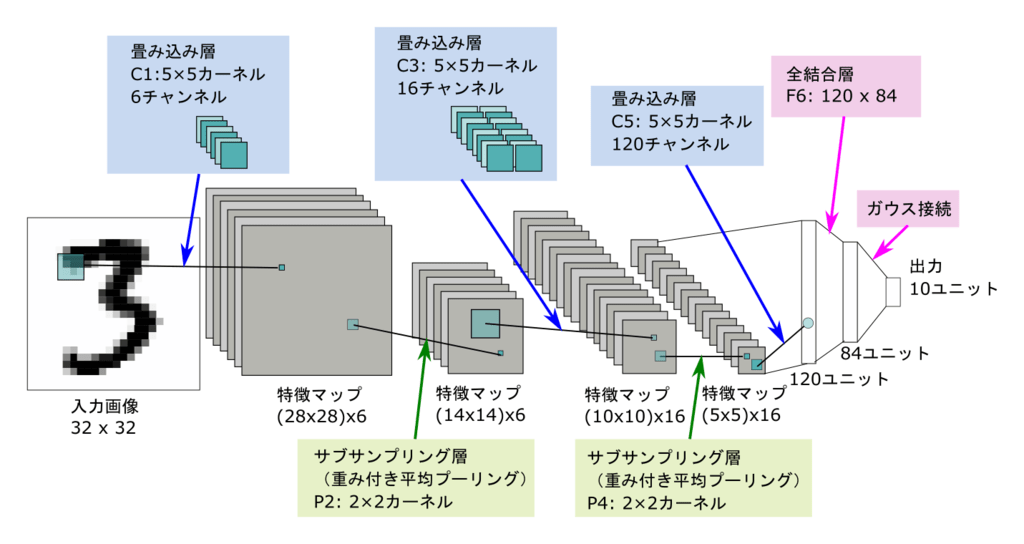
\includegraphics[width=14cm]{./capture/LeNet.png}
    \caption{LeNetの概要(https://cvml-expertguide.net/terms/dl/cnn/cnn-backbone/lenet/より引用)}
    \label{fig:lenet}
\end{figure}
  
\newpage

\subsection{畳み込み(Convolution)層}
CNNでは、LeNet同様、畳み込み層、プーリング層、全結合層から構成される。
CNNにおける畳み込み層では、フィルタ(カーネルとも呼ぶ)を用いて、画像という大きな行列の特徴を抽出する。
フィルタは、画像の一部分に対して「重みのかけ合わせ = 畳み込み」を行い、画像の特徴を抽出するための行列である。
\begin{align}
  u_{ij} = \sum^{w_f}_{p=0} \sum^{h_f}_{q=0} x_{i+p, j+q}w_{pq}
\end{align}
ここで、$u_{ij}$は出力画像のピクセル値、$x_{i+p, j+q}$は入力画像のピクセル値、$w_{pq}$はフィルタの重み、$w_f, h_f$はフィルタの幅と高さである。
\par
この積和演算を画像全体に対して行うことで、画像の特徴を抽出することができる。
畳み込みでは、次元の繋がりを保ちながら、画像の特徴を抽出するために、フィルタをスライドさせて、画像全体に対して演算を行う。フィルタの数は、画像の特徴を抽出するための次元数であり、フィルタの数が多いほど、画像の特徴を多く抽出することができる。図\ref{fig:convolution_layer}に畳み込み層の概念図を示す。
\par
畳み込み層における主要なハイパーパラメータには、以下のようなものがある。
\begin{itemize}
  \item パディング
  \item ストライド
  \item チャンネル
\end{itemize}
\par
パディングは、画像の次元を保つために画像の端にハイパーパラメータを追加することである。
パディングを行うことで、画像の端の特徴も抽出することができる。
\par
ストライドは、フィルタをスライドさせる幅を表すハイパーパラメータである。
ストライドを大きくすることで、画像の次元を小さくすることができる。
\par
チャンネルは、フィルタの数を表すハイパーパラメータである。
チャンネルを増やすことで、画像の特徴を多く抽出することができる。

\begin{figure}
  \centering
  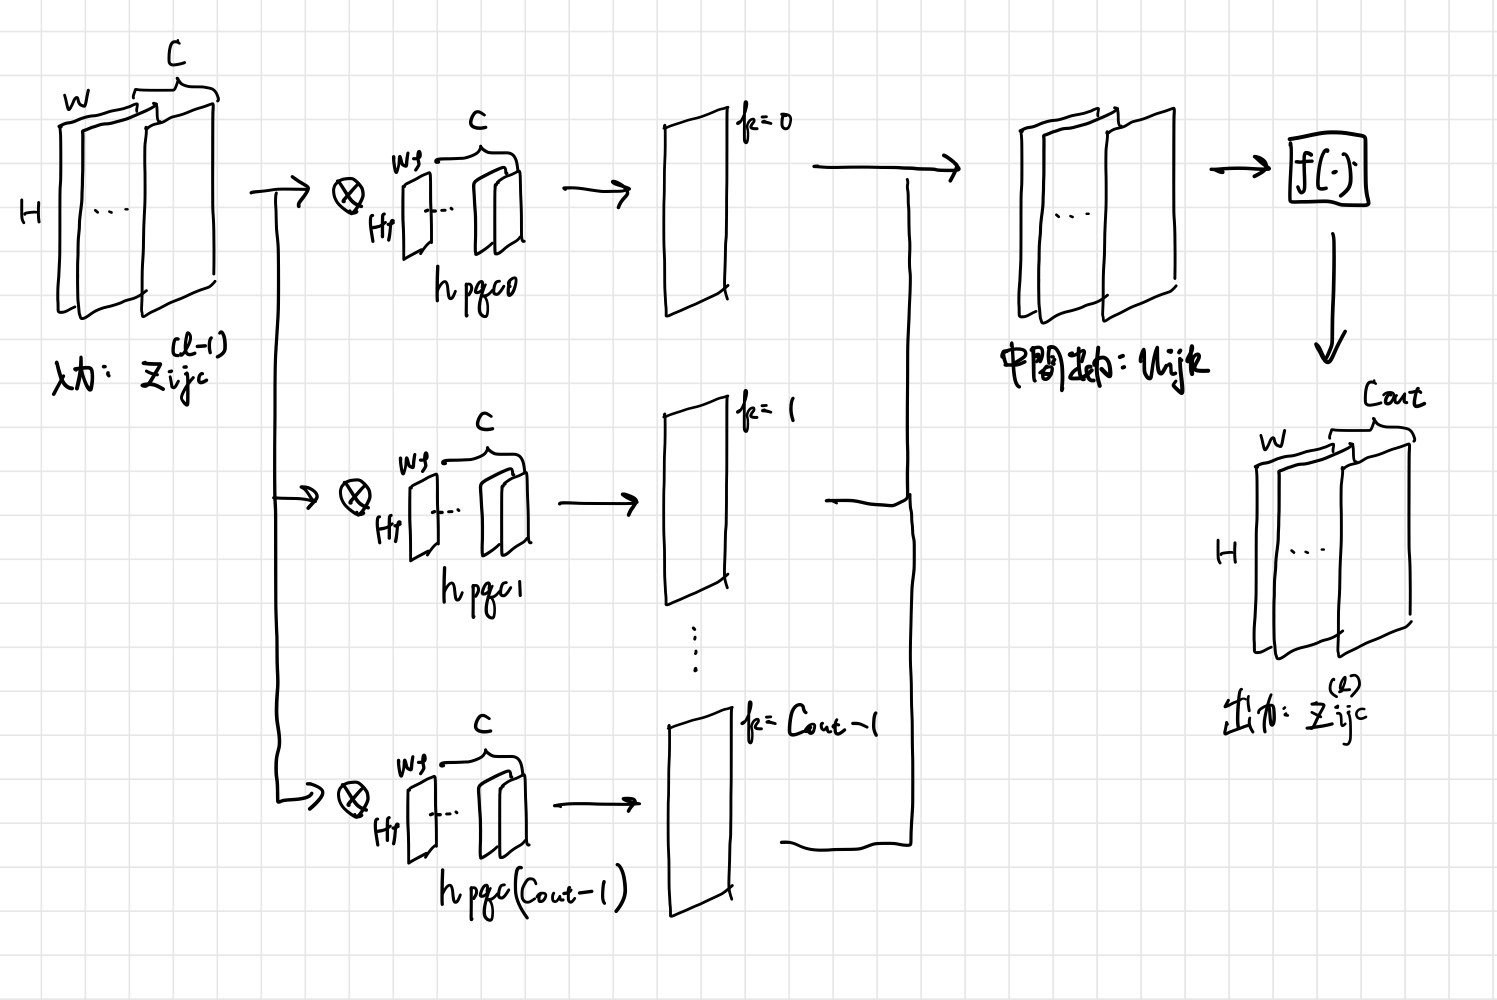
\includegraphics[width=12cm]{./capture/Convolution_layer.png}
  \caption{畳み込み層の概念図. この畳み込み層は$W\times H \times C$の入力に対し、$C_{\text{out}}$個のフィルタ(縦横 $W_f\times H_f \times C$)を適用し、$W\times H \times C_{\text{out}}$の出力を得る.}
  \label{fig:convolution_layer}
\end{figure}

\begin{itembox}[l]{確認テスト}
  Q: サイズ6×6の入力画像を、サイズ2×2のフィルタで畳み込んだ時の出力画像のサイズを答えよ。なおストライドとパディングは1とする。
 
  A: 出力画像は5×5となる。なぜなら、ストライド1の時、フィルタをスライドさせる間隔は1つずつで、パディングが1の時、入力画像の周囲に1マスずつ余白が生じるためである。\\
  なお、公式は以下の通りとなる。

  \begin{align}
    \frac{{\text{入力画像のサイズ}} + 2 \times \text{パディング} - \text{フィルタサイズ}}{{\text{ストライド}}} + 1
  \end{align}
 
\end{itembox}

\subsection{プーリング(pooling)層}
一般的にプーリング層では2つの役割がある。1つは、入力の各位置でその局所領域内の値を要約することであり、もうひとつは入力の空間解像度を下げるダウンサンプリングの実行である。
要約の仕方は、畳み込んだ行列の中で最大の値を取り出したり、平均値を取り出すなどがある。
この時、前者の方法をMaxプーリング、 後者の方法をAverageプーリングと呼ぶ。


\subsection{全結合層}
全結合層は、畳み込み層やプーリング層で抽出した特徴を元に、最終的な出力を行う層である。
全結合層では、畳み込み層やプーリング層で抽出した特徴を1次元のベクトルに変換し、出力層に渡す。
1次元への変換は、Flatten, Global MaxPooging, Global AveragePoolingなどの手法がある。
Flattenは、抽出した特徴をすべて1次元のベクトルに変換する手法である
Global MaxPoolingは、抽出した特徴の中から1チャンネルの中での最大の値を取り出す手法である。
Global AveragePoolingは、抽出した特徴の中から1チャンネルの中での平均値を取り出す手法である。


\subsection{AlexNet}
AlexNetは、深層学習による画像認識ブームの火付け役となったモデルである。
224×224の画像を入力とし、55×55の畳み込み層、27×27のプーリング層、13×13の畳み込み層、6×6のプーリング層、全結合層、出力層から構成される。
AlexNetでは、以下の工夫を行ったことで、誤差が大幅に削減され、高い性能を発揮した。
\begin{enumerate}
  \item ReLU関数の導入
  \item ドロップアウトの導入
  \item データ拡張
  \item バッチ正規化
\end{enumerate}

それまでのCNNでは、シグモイド関数やハイパボリックタンジェント関数を活性化関数として用いていたが、これらの関数を用いた場合、層を増やした時に微分値が小さくなるため、勾配が爆発したり消失する問題があった。
ReLU関数は、そのような問題を解決するために導入された関数であり、勾配が消失しないため、層を深くすることができた。

\newpage

\section{day3 : 再帰型ニューラルネットワーク(RNN)}
\subsection{概要}
RNNは、時系列データを扱う際に有効なニューラルネットワークである。
時系列データとは、時間的順序を追って一定間隔毎に観測され、相互に統計的依存関係が認められるようなデータの系列のことである。
例えば、音声データ、テキストデータ、株価データなどが挙げられる。
(テキストデータが時系列データとなるのは、単語の並び順によって文章が構築されるためである。)
RNNは、時系列データの特徴を捉えるために、中間層の出力が次の時刻の入力として用いられる。

\subsection{RNNにおける順伝搬}
以降では、RNNの基本的な構造について説明するため、系列$\mathbf{x_1}, \mathbf{x_2}, \cdots$ をRNNに順番に入力したときに、対応する出力$\mathbf{y_1}, \mathbf{y_2}, \cdots$ を得ることを考える。
まず、入力層・中間層・出力層の各ユニットのインデックスを$i, j, k$とする。そして、時刻$t$における中間層ユニットへの出力を$\mathbf{u^t} = (u^t_j)$と$\mathbf{z^t} = (z^t_j)$、出力層のユニットへの出力を$\mathbf{v^t} = (v^t_k)$ と $\mathbf{y_t}=(y^t_k)$とする。入力層と中間層間の重みを$W^{\text{(in)}} = W^{\text{(in)}}_{ji}$、中間層から中間層への重みを$W = (W_{jj'})$、中間層と出力層間の重みを$W^{\text{(out)}} = W^{\text{(out)}}_{kj}$とする。

この時、時刻$t$における中間層$j$ユニットへの出力$u^t_j$は、以下のように表される。
\begin{align}
  u^t_j = \sum_{i} W^{\text{(in)}}_{ji}x^t_i + \sum_{j'} W_{jj'}z^{t-1}_{j'}
\end{align}
これは、時刻$t$における中間層の各ユニットへの入力が、入力層からの入力と、前の時刻$t-1$における中間層の出力からの入力の和であることを示している。ここでは、$W^{\text{(in)}}_{j0}$ をバイアスとして与えている。
以上の導出過程の概略図を図\ref{fig:RNN_forward}に示す。
\begin{figure}[htbp]
  \centering
  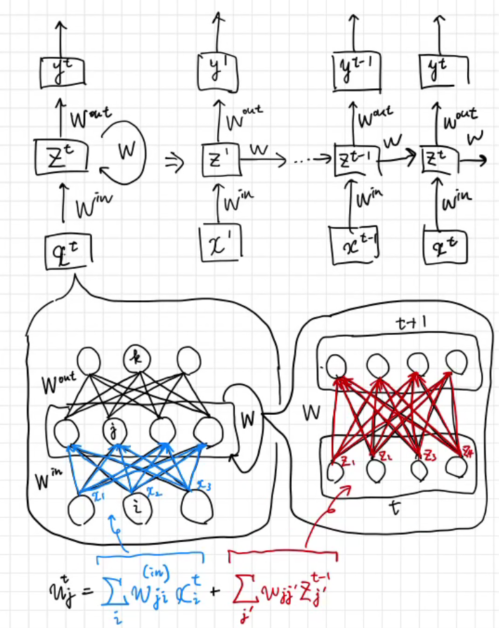
\includegraphics[width=13cm]{./capture/RNN.png}
  \caption{RNNにおける順伝搬の概略図}
  \label{fig:RNN_forward}
\end{figure}

活性化関数を$f(u^t_j)$とすると、中間層の出力$z^t_j$は、
\begin{align}
  z^t_j = f(u^t_j)
\end{align}
となる。これらをまとめると、時刻$t$における中間層の入力$\mathbf{u^t}$、出力$\mathbf{z^t}$、出力層の入力$\mathbf{v^t}$、出力$\mathbf{y^t}$は、
\begin{align}
  \mathbf{u^t} &= \mathbf{W^{\text{(in)}}}\mathbf{x^t} + \mathbf{Wz^{t-1}}\\
  \mathbf{z^t} &= f(\mathbf{W^{\text{(in)}}}\mathbf{x^t} + \mathbf{Wz^{t-1}})\\
  \mathbf{v^t} &= \mathbf{W^{\text{(out)}}}\mathbf{z^t} + c\\
  \mathbf{y^t} &= g(\mathbf{W^{\text{(out)}}}\mathbf{z^t} + c)
\end{align}
となる。ただし、$c$は出力層のバイアスである。また、$g$は出力層の活性化関数である。



\subsection{RNNにおける誤差逆伝播法}
RNNで誤差逆伝播法を用いて重みを更新する際には、RTRL(Real Time Recurrent Learning)やBPTT(Back Propagation Through Time)といった手法が用いられる。前者はメモリ効率が良く、後者は計算効率が良いという特徴がある。ここではBPTTについて説明する。

RNNでは、時刻$t$の中間層$j$の入力$u_j^t$を以下で表した。
\begin{align}
  u_j^t = \sum_i W_{ji}^{\text{(in)}}x_i^t + \sum_{j'} W_{jj'}z_{j'}^{t-1}
\end{align}
これは、時刻$t$における入力層からの入力$x_i^t$と、時刻$t-1$における中間層の出力$z_{j'}^{t-1}$からの入力に各重み成分を掛け合わせたの和としてあらわされている。

ここで、ニューラルネットワークの逆伝播では以下のように表せた。
\begin{align}
  \frac{\partial E}{\partial w_{ji}} &= \sum_t \frac{\partial E}{\partial u_j^t} \frac{\partial u_j^t}{\partial w_{ji}}\\
  &= \sum_t \delta_j^t z_i^t
\end{align}
ただし、$\delta_j^t$は中間層$j$の誤差であり、以下のように表される。
\begin{align}
  \delta_j = \frac{\partial E}{\partial u_j} = \frac{\partial E}{\partial z_j} \frac{\partial z_j}{\partial u_j}
\end{align}

RNNにおける$\delta_j^t$は、時刻$t$における出力層$k$の入力$v_k^t$と、時刻$t+1$における中間層$j'$の入力$u_{j'}^{t+1}$に依存するため、以下のように表される。
\begin{align}
  \delta_j^t &= \frac{\partial E}{\partial u_j^t}\\
   &= \sum_k \frac{\partial E}{\partial v_k^t} \frac{\partial v_k^t}{\partial u_j^t} + \sum_{j'} \frac{\partial E}{\partial u_{j'}^{t+1}} \frac{\partial u_{j'}^{t+1}}{\partial u_j^t}
\end{align}
まず、前半部分は、以下のように展開できる。
\begin{align}
  \sum_k \frac{\partial E}{\partial v_k^t} \frac{\partial v_k^t}{\partial u_j^t} &= \sum_k \delta_k^t \frac{\partial v_k^t}{\partial u_j^t}\\
  &= \sum_k \delta_k^t \frac{\partial}{\partial u_j^t} \left( \sum_{j} W_{kj}^{\text{(out)}}z_{j}^t + c \right)\\
  &= \sum_k \delta_k^t W_{kj}^{\text{(out)}} \frac{\partial z_j^t}{\partial u_j^t}\\
  &= \sum_k \delta_k^t W_{kj}^{\text{(out)}} \frac{\partial g(u_j^t)}{\partial u_j^t}\\
  &= \sum_k \delta_k^t W_{kj}^{\text{(out)}} g'(u_j^t)
\end{align}

そして、後半部分は、以下のように展開できる。
\begin{align}
  \sum_{j'} \frac{\partial E}{\partial u_{j'}^{t+1}} \frac{\partial u_{j'}^{t+1}}{\partial u_j^t} &= \sum_{j'} \delta_{j'}^{t+1} \frac{\partial u_{j'}^{t+1}}{\partial u_j^t}\\
  &= \sum_{j'} \delta_{j'}^{t+1} \frac{\partial}{\partial u_j^t} \left( \sum_i W_{j'i}^{\text{(in)}}x_i^{t+1} + \sum_{j} W_{j'j}z_{j}^t \right)\\
  &= \sum_{j'} \delta_{j'}^{t+1} \frac{\partial}{\partial u_j^t} \left( \sum_i W_{j'i}^{\text{(in)}}x_i^{t+1} + \sum_{j} W_{j'j}f(u_j^t) \right)\\
  &= \sum_{j'} \delta_{j'}^{t+1} W_{j'j} f'(u_j^t)
\end{align}
よって、$\delta_j^t$は以下のように表される。
\begin{align}
  \delta_j^t =  \sum_k \delta_k^t W_{kj}^{\text{(out)}} g'(u_j^t) + \sum_{j'} \delta_{j'}^{t+1} W_{j'j} f'(u_j^t)
\end{align}

この結果を用いて、誤差関数を各重みで微分した値を導出できる。
\begin{align}
  \frac{\partial E}{\partial W_{ji}^{\text{(in)}}} &= \sum_{t=1}^T \frac{\partial E}{\partial u_j^t} \frac{\partial u_j^t}{\partial W_{ji}^{\text{(in)}}}\\
  &= \sum_{t=1}^T \delta_j^t x_i^t
\end{align}
\begin{align}
  \frac{\partial E}{\partial W_{jj'}} &= \sum_{t=1}^T \frac{\partial E}{\partial u_j^t} \frac{\partial u_j^t}{\partial W_{jj'}}\\
  &= \sum_{t=1}^T \delta_j^t z_{j'}^{t-1}
\end{align}
\begin{align}
  \frac{\partial E}{\partial W_{kj}^{\text{(out)}}} &= \sum_{t=1}^T \frac{\partial E}{\partial v_k^t} \frac{\partial v_k^t}{\partial W_{kj}^{\text{(out)}}}\\
  &= \sum_{t=1}^T \delta_k^t z_j^t
\end{align}

\begin{itembox}[l]{確認テスト}
  Q: 図\ref{fig:day3_07_1}について、$y_1$を、$x, z_0, z_1, W_{\text{(in)}}, W, W_{\text{(out)}}$を用いて数式で表せ。

  A: 以下導出の通り。ただし、$g$は活性化関数、$c$はバイアスである。
  \begin{align}
    y_1 &= \sum W_{\text{(out)}}z_1 + c\\
    &= \sum W_{\text{(out)}}g(\sum Wz_0 + \sum W^{\text{(in)}}x + c) + c
  \end{align}
\end{itembox}

\begin{figure}
  \centering
  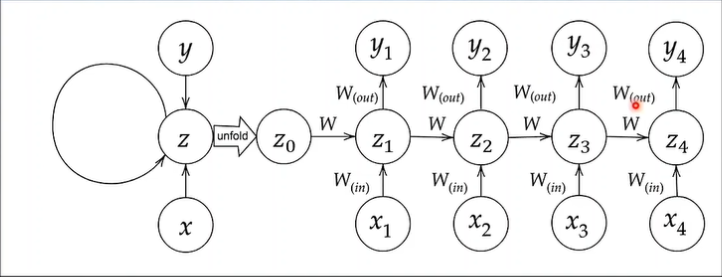
\includegraphics[width=10cm]{./capture/confirm_test/day3_07_1.png}
  \caption{}
  \label{fig:day3_07_1}
\end{figure}

\subsection{LSTM}
RNNは、時刻$t$における一つのニューラルネットワークを、$t=0$から$t=T$まで繰り返し適用するモデルである。
一つのニューラルネットワークでさえ、逆伝播において勾配消失問題について考える必要があるが、RNNでは、時刻が進むにしたがってより多くのニューラルネットワークを重ねていくため、逆伝播における勾配消失問題がより顕著になる。
また、逆に、時刻が進むにしたがって逆伝播における勾配が爆発する問題も発生する。
\begin{itembox}[l]{確認テスト}
  Q: RNNや深いモデルでは勾配の消失や爆発が起こる傾向がある。勾配爆発を防ぐために勾配のクリッピングという手法が使われることがある。具体的には勾配のノルムが閾値を超えたら、勾配のノルムを閾値に正規化するというものである。この関数を完成させなさい。

  A: 
  \begin{verbatim}
    def gradient_clipping(grad, threshold):
      norm = np.linalg.norm(grad) # 勾配のノルムを計算
      rate = threshold / norm
      if rate < 1:
        return grad * rate 
      return grad
  \end{verbatim}  

\end{itembox}

この問題を解決するために、LSTM(Long Short-Term Memory)が提案された。
図\ref{fig:LSTM}にLSTMの構造を示す。
\begin{figure}[htbp]
  \centering
  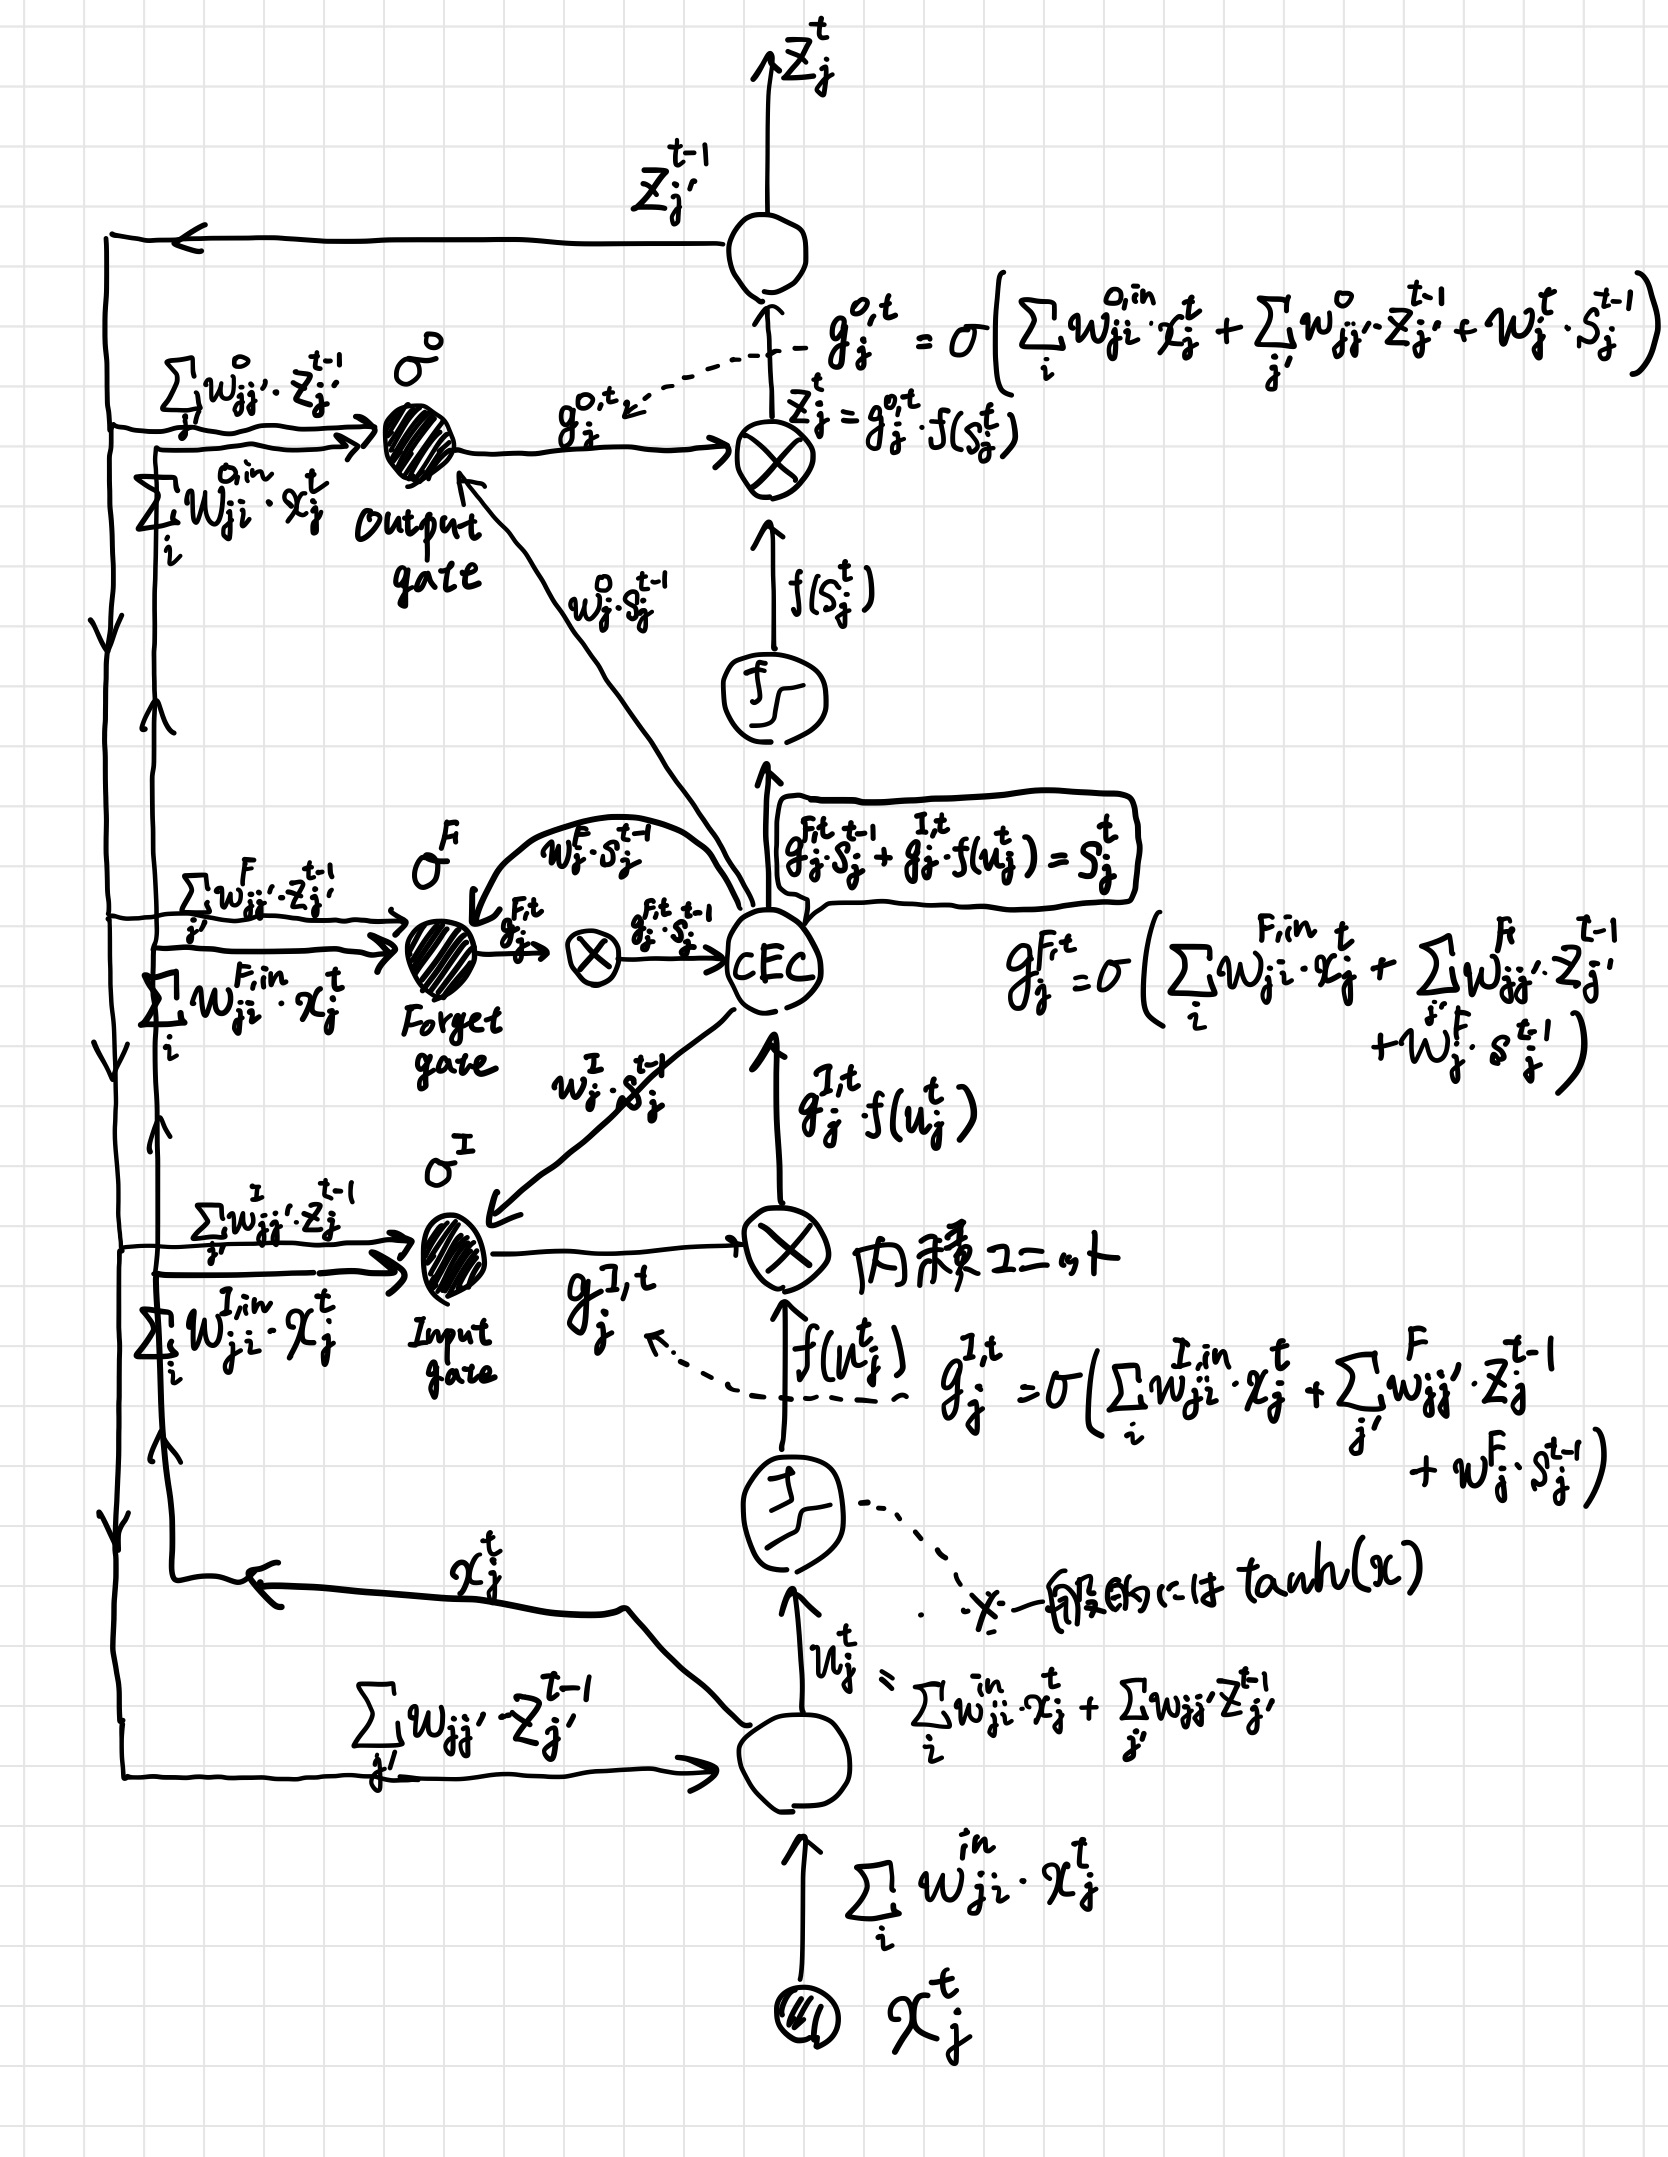
\includegraphics[width=13cm]{./capture/LSTM-33.jpg}
  \caption{LSTMの構造}
  \label{fig:LSTM}
\end{figure}

\newpage

図\ref{fig:LSTM}によれば、入力ゲート・出力ゲート・忘却ゲートの3つのゲートが存在し、入力・出力ゲートは層と層の間に設けられ、忘却ゲートはCEC(Constant Error Carrousel)と呼ばれる、過去の情報を保持するためのユニットとループ状態で接続されている。
\subsubsection{CEC}
CECは記憶を保持するためのユニットであり、学習機能有さない。学習の機能は各種ゲートによって制御され、CECに何を覚えさせるか、何を忘れさせるか、何を出力するかを制御する。
\subsubsection{入力ゲート}
入力ゲートでは、時刻$t$の入力$x_j^t$と、時刻$t-1$の出力$z_j^{t-1}$、そして、時刻$t-1$のCECの情報$s_j^{t-1}$の3つを入力として、新しい情報をCECに追加する。$x_j^t$, $z_j^{t-1}$, $s_j^{t-1}$に対してはそれぞれの別の重みが掛けられ、情報を重視する割合を調整する。この重みが学習によって最適化される。
\subsubsection{出力ゲート}
出力ゲートでは、時刻$t$の入力$x_j^t$と、時刻$t-1$の出力$z_j^{t-1}$、そして、時刻$t$CECの情報$s_j^{t}$の3つを入力として、最終的に出力する値の調整を行う。こちらにも割合を調整する重みが掛けられ、学習によって最適化される。
\subsubsection{忘却ゲート}
忘却ゲートでは、時刻$t$の入力$x_j^t$と、時刻$t-1$の出力$z_j^{t-1}$、そして、時刻$t-1$CECの情報$s_j^{t-1}$の3つを入力として、CECの情報をどれだけ忘れるかを調整する。もし、忘却ゲートが無かったら、過去の情報が無限に保持されることになる。このことは過去の情報がいらなくなった場合に、削除することができないことを意味する。忘却ゲートによって、過去の情報を必要な時に保持し、不要な時に削除することができる。これによって、勾配消失や勾配爆発を防ぐことができる。

\newpage

\begin{itembox}[l]{確認テスト}
  Q: 以下の文章をLSTMに入力し空欄に当てはまる単語を予測したいとする。文中の「とても」という言葉は空欄の予測において無くなっても影響を及ぼさないと考えられる。このような場合、どのゲートが作用すると考えられるか。
  \par
  「映画おもしろかったね。ところで、とてもお腹が空いたから何か\_\_\_\_\_。」

  A: 忘却ゲートが作用する。忘却ゲートによって過去の情報の有無を判断しているため、「とても」という単語の影響が少ないことを学習することができる。

  Q: LSTMの順伝搬を行うプログラムを書け。

  A: 以下に示す。
  \begin{verbatim}
    def lstm(x, prev_h, prev_c, W, U, b):
      """
      x: inputs, (batch_size, input_size)
      prev_h: previous output at time t-1, (batch_size, hidden_size)
      prev_c: previous cell state at time t-1, (batch_size, hidden_size)
      W: upwrad weights, (4*state_size, input_size)
      U: lateral weights, (4*state_size, hidden_size)
      b: biases, (4*state_size,)
      """

      # セルへの入力やゲートをまとめて計算し分割する
      a = np.dot(x, W.T) + np.dot(prev_h, U.T) + b
      a, ai, af, ao = np.split(a, 4, axis=1)

      # 各ゲートの計算
      ig = sigmoid(ai)
      fg = sigmoid(af)
      og = sigmoid(ao)

      # セルの値の計算
      c = fg * prev_c + ig * np.tanh(a) # 要素同士の積を求めるため、np.dotにはならないことに注意
      h = og * np.tanh(c)

      return h, c
  \end{verbatim}
\end{itembox}

\newpage

\subsection{GRU(Gated Recurrent Unit)}
LSTMでは、パラメータ数が多く、計算コストが高いという問題があった。この問題を解決するために、GRUが提案された。
GRUでは、LSTMの入力ゲートと忘却ゲートを「更新ゲート」として統合し、また、出力ゲートを廃止することで、パラメータ数を削減している。また、「リセットゲート」を導入することで、過去の情報をどれだけ保持するかを調整することができる。
CECへの入力値$\mathbf{u^t}$, CECの保持値$\mathbf{s^{t}}$, 出力$\mathbf{z^t}$は以下のように表される。
\begin{align}
  \label{eq:GRU1}
  \mathbf{u^t} &=\mathbf{W^{\text{(in)}}}\mathbf{x^t} + \mathbf{Wg}^{R,t} \odot z^{t-1}\\
  \mathbf{s^t} &= \mathbf{g}^{U,t} \odot \mathbf{s^t} + (1 - \mathbf{g}^{U,t}) \odot f(\mathbf{u^t})\\
  \mathbf{z^t} &= \mathbf{s^t}
\end{align}
ここで、$\odot$は要素積を表す。また、$\mathbf{g}^{R,t}$はリセットゲート、$\mathbf{g}^{U,t}$は更新ゲートの出力値で、
\begin{align}
  \mathbf{g}^{R,t} &= \sigma(\mathbf{W^R}\mathbf{x^t} + \mathbf{U^R}\mathbf{z^{t-1}})\\
  \mathbf{g}^{U,t} &= \sigma(\mathbf{W^U}\mathbf{x^t} + \mathbf{U^U}\mathbf{z^{t-1}})
\end{align}
と表される。$\sigma$はシグモイド関数である。
式\eqref{eq:GRU1}の右辺第二項の$\mathbf{g}^{R,t}$が無かった時、更新ゲートの値が0であった場合に、過去の状態が常に同じ割合($\mathbf{Wz^{t-1}}$)で現在に伝播されてしまうが、リセットゲートを導入することで、忘却ゲートのように過去の情報をどれだけ保持するかを調整することができる。

\subsection{双方向RNN}
双方向RNNは、時系列データを前方向と後方向の2つのRNNで処理し、それぞれの出力を結合することで、より正確な予測を行うことができる。文章の推敲や、機械翻訳などで利用される。
双方向RNNのPythonコードを以下に示す。
\begin{itembox}[l]{}
\begin{verbatim}
  import numpy as np

  def bidriectinoal_rnn(xs, W_f, U_f, W_b, U_b, V):
  """
  W_f, U_f : forward rnn weights, (hidden_size, input_size)
  W_b, U_b : backward rnn weights, (hidden_size, input_size)
  V: output weights, (output_size, hidden_size)
  """

    xs_f = np.zeros_like(xs)
    xs_b = np.zeros_like(xs)
    for i , x in enumerate
      xs_f[i] = x
      xs_b[i] = x[::-1]
    hs_f = forward_rnn(xs_f, W_f, U_f)
    hs_b = forward_rnn(xs_b, W_b, U_b)
    hs = [np.concatenate([h_f, h_b[::-1]], axis=1) for h_f, h_b in zip(hs_f, hs_b)]
    ys = hs.dot(V.T)
    return ys
\end{verbatim}
\end{itembox}
ここで、numpyのconcatenateは、配列を結合する関数である。具体的には、axis=0の場合、縦方向に結合し、axis=1の場合、横方向に結合する。そのあとのzip関数は、複数のリストを同時にループ処理するための関数である。こうすることで、過去と未来の情報を無くすこと無く、演算することができる。


\subsection{自己回帰モデル}
自己回帰モデルは、時系列データを入力し、その出力を次の時刻の入力として再帰的に処理するモデルである。RNNは、自己回帰モデルの一種である。
\begin{align}
  \mathbf{x}^t = \phi_0 + \sum_{i=t-\rho}^{t-1} \phi_i \mathbf{x}^i + \epsilon^t
\end{align}
ここで、$\phi_0$は定数項、$\phi_i$は係数、$\epsilon^t$はノイズである。この式は、時刻$t$における入力$\mathbf{x}^t$が、過去の入力$\mathbf{x}^{t-1}, \mathbf{x}^{t-2}, \cdots$に依存していることを示している。

\subsection{Seq2Seq}
Seq2Seqは、時系列データを入力として、長さの異なる時系列データを出力するモデルである。機械翻訳や対話モデルなどで利用される。
Seq2Seqの構造は、図\ref{fig:Seq2Seq}のようになる。
\begin{figure}[htbp]
  \centering
  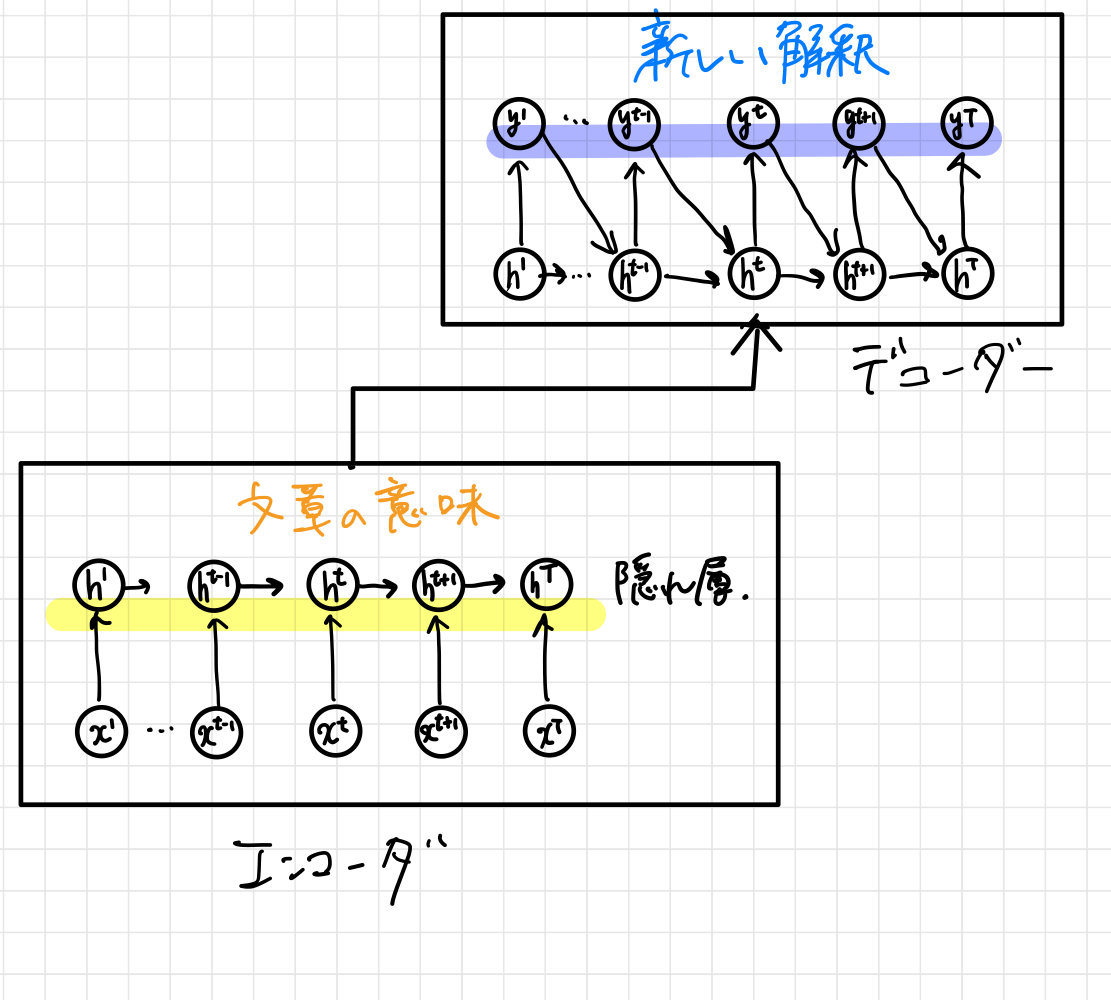
\includegraphics[width=13cm]{./capture/Seq2Seq.png}
  \caption{Seq2Seqの構造}
  \label{fig:Seq2Seq}
\end{figure}

Seq2Seqは、エンコーダとデコーダから構成される。エンコーダは、入力データを受け取り、中間層の出力をデコーダに渡す。デコーダは、エンコーダから受け取った中間層の出力を元に、出力データを生成する。エンコーダとデコーダは、LSTMやGRUなどのRNNを用いて構築される。

\subsubsection{Encoder RNN}
エンコーダでは、主に、Taking, Embedding, RNNの3つの処理を行う。
Takingでは、ユーザーがインプットしたデータを単語毎に分割する。
\par
Embeddingでは、分割した単語をベクトルに変換する。例えば英語なら、英単語のうち代表的なものを$K$語選び、これを 1-of-$K$符号化する。これをEmbedding Matrixと呼ぶ。その後、入力に対して各単語に対応するベクトルを生成する。このベクトルは、似た単語の意味は似た配列となるように機械学習によって生成される。
\par
RNNでは、Embeddingで生成されたベクトルを入力として受け取る。例えば、文章の途中を隠して単語を予測したり、後に続く文章を生成したりすることができる。

\subsubsection{Decoder RNN}
Encoderの内部状態を入力して、出力を生成する。この時、用いるEmbedding Matrixは、必ずしもEncoderで利用した$K$語の単語である必要はなく、異なる言語のEmbedding Matrixを用いることもできる。こうすることで、異なる言語間での翻訳が可能となる。

\subsubsection{HRED}
HRED(Hierarchical Recurrent Encoder-Decoder)は、Seq2Seqの拡張モデルである。Seq2Seqでは、文脈を考慮した応答ができないという問題があったが、HREDでは、文脈を考慮した応答が可能となる。
Seq2Seqにおけるエンコーダの中間層の出力を、さらに過去のエンコーダ出力とRNNと繋いで処理する。この、会話コンテキスト全体を表すベクトルをContext RNNと呼ぶ。
\par
ただし、HREDは同じコンテキストが与えられた場合に、同様の出力になってしまったり、短い返答を学んでしまう問題があった。この問題を解決するために、VHRED(Variational Hierarchical Recurrent Encoder-Decoder)が提案された。VHREDは、HREDにVAE(Variational Auto-Encoder)を組み合わせたモデルである。VAEは、データの生成過程を確率モデルとして表現し、データの生成過程を学習するモデルである。VHREDは、HREDの中間層の出力をVAEの入力として、文脈を考慮した応答を生成する。

\subsection{VAE(Variational Auto-Encoder)}
\subsubsection{オートエンコーダ}
オートエンコーダーは、教師無し学習を用いて、入力と出力が同じ値になるように、エンコーダとデコーダを作成していく、教師無し学習の一つである。
入力と潜在変数の間にはエンコーダが、出力と潜在変数の間にはデコーダが存在する。エンコーダによって入力データを次元削減し、特徴を抽出する。デコーダによって、次元削減されたデータを元の次元に戻す。この時、入力と出力が同じになるように学習を行う。

\subsection{word2vec}
word2vecは、単語をベクトルに変換する手法である。word2vecには、CBOW(Continuous Bag of Words)とSkip-gramの2つの手法がある。
CBOWは、周囲の単語から中央の単語を予測するモデルである。Skip-gramは、中央の単語から周囲の単語を予測するモデルである。
word2vecは、単語の意味をベクトル化することができるため、自然言語処理の分野で広く利用されている。

\subsection{Attention Mechanism}
Attention Mechanismは、Seq2Seqの問題点である、長い文章を処理する際に、過去の情報が失われてしまう問題を解決するために提案された。Attention Mechanismは、入力データの各単語に重みを付け、重要な単語に大きな重みを付けることで、過去の情報を保持することができる。


\paragraph{参考文献}
\begin{enumerate}
  \item 岡谷貴之/深層学習 改訂第2版 [機械学習プロフェッショナルシリーズ]/ 講談社サイエンティフィク/ 2022-01-17
  \item RNN入門PART1$\sim$3/@\_livesomewhere1090 \url{https://www.youtube.com/@\_livesomewhere1090}
\end{enumerate}

以下、レポート及びステージテストの参考文献
\begin{enumerate}
  \item [DeepLearning] 計算グラフについて理解する/@edo\_m18(Kazuya Hiruma) \url{https://qiita.com/edo_m18/items/7c95593ed5844b5a0c3b}
  \item 誤差逆伝播法を計算グラフを使って分かりやすく解説する \url{https://deepage.net/deep\_learning/2017/04/02/backpropagation.html}
  \item 交差エントロピー誤差をわかりやすく説明してみる/@kenta1984(Kenta Sasaki) \url{https://qiita.com/kenta1984/items/59a9ef1788e6934fd962}
  \item カーネル関数って結局なんなの?→サンプル間の類似度と理解するのがよいと思います! \url{https://datachemeng.com/what_is_kernel/}
  \item LeNet: 最初のCNN構造 \url{https://cvml-expertguide.net/terms/dl/cnn/cnn-backbone/lenet/}
  \item AlexNet: 大規模な画像物体認識むけCNNの元祖 \url{https://cvml-expertguide.net/terms/dl/cnn/cnn-backbone/alexnet/#3_AlexNet_\%E3\%81\%AE\%E7\%89\%B9\%E5\%BE\%B4\%E3\%83\%BB\%E5\%B7\%A5\%E5\%A4\%AB}
\end{enumerate}

\newpage
\end{document}